\documentclass[a4paper]{article}
\usepackage{hyperref}
\usepackage{xcolor}
\usepackage{graphicx}
\usepackage{float}
\usepackage[export]{adjustbox}
\usepackage[english]{babel}
\usepackage[T1]{fontenc}
\usepackage{url}
\usepackage{import}
\usepackage{multirow}
\usepackage{color}
\usepackage{fancyhdr}
\usepackage{amssymb}
\usepackage{tabu}
\usepackage{mathtools}
\usepackage[margin=2.5cm]{geometry}
\usepackage{listings}
\usepackage{titling}
\usepackage[utf8]{inputenc}
\usepackage[numbered,framed]{matlab-prettifier}
\usepackage{amsmath}
\usepackage{animate}
\usepackage[labelformat=empty]{caption}

\let\ph\mlplaceholder
\lstMakeShortInline"

\newcommand{\bnb}{\begin{nobreak}}
\newcommand{\enb}{\end{nobreak}}

\lstset{
	style              = Matlab-editor,
  	basicstyle         = \mlttfamily,
  	escapechar         = ",
  	mlshowsectionrules = true,
}

\pretitle{
	\begin{center}
  		\LARGE
  		
\includegraphics[width=\textwidth/4]{assets/logo-unifi.png}\\[\bigskipamount]
}
\posttitle{\end{center}}

\title{\vspace{2cm}Elaborato di\\ \textbf{Calcolo Numerico}\\ Anno Accademico 2017/2018\vspace{1cm}}

\author
{Mattia D'Autilia - \texttt{5765968} mattia.dautilia@stud.unifi.it\\Yuri Bacciarini - \texttt{5654547} yuri.bacciarini@stud.unifi.it}

\date{}

\addto\captionsenglish{\renewcommand{\contentsname}{Capitoli}}

\begin{document}

\pagenumbering{Roman}
	
\maketitle

\begin{center}
	\today{}
\end{center}

\newpage

\newpage

\tableofcontents
\newpage

\pagenumbering{arabic}

\section{\textbf{Capitolo 1}}
\subsection{Esercizio 1}
Volendo conoscere quanto un errore influenzi il risultato quando $x\neq0$, si definisce l’errore relativo:
\[
|\epsilon_x| = \frac{\tilde{x}-x}{x} 
\]
da cui :
\[
\tilde{x} = x(1+\epsilon_x), \text{ e quindi } \frac{\tilde{x}}{x} = 1 + \epsilon_x
\]
ovvero l’errore relativo deve essere comparato a 1: un errore relativo vicino a zero indicherà che il risultato approssimato è molto vicino al risultato esatto,mentre un errore relativo uguale a 1 indicherà la totale perdita di informazione.\\\\
Con $x = e \approx 2.7183 = \tilde{x}, \text{l'errore relativo è quindi } |\epsilon_x| = \frac{2.7183 - e}{e} = 6.6849e-06$\\\\
Il numero di cifre significative \textit{k} corrette all’interno di $\tilde{x}$ si definisce con la formula :
\[
\textit{k} = -\log(2|\epsilon_x|)
\]
In questo caso il risultato del calcolo è $\textit{k}=4.8739$, che è abbastanza vicino alla realtà di $\textit{k}=5$ cifre significative corrette.\\\\
Spesso, per avere un’idea di quanto è l’ordine di grandezza di $\epsilon$ si scrive:
\[
|\epsilon_x| \approx \frac{1}{2}10^{-\textit{k}}
\]
infatti : 
\[
|\epsilon_x| \approx \frac{1}{2}10^{-4.8739} = 6.6849e-06 = |\epsilon_x|
\]
\subsection{Esercizio 2}
Partiamo da :
	\[
	f'(x) \approx \frac{f(x+h) - f(x-h)}{2h}
	\]
Usando gli sviluppi di Taylor fino al secondo ordine otteniamo:
	\[
	f(x+h) = f(x) + f'(x)h + \frac{1}{2} f''(x)h^{2} + \frac{1}{6}f'''(\xi_x)h^{3}
	\]
	\[f(x-h) = f(x) - f'(x)h + \frac{1}{2} f''(x)h^{2} - \frac{1}{6}f'''(\mu_x)h^{3}
	\]
Al numeratore otteniamo
	\[
	f(x+h) - f(x-h) = 2f'(x)h + \frac{1}{6}(f'''(\xi_x)h^{3}+f'''(\mu_x)h^{3})
	\]
La relazione iniziale diventa
	\[
	f'(x) \approx \frac{f(x+h) - f(x-h)}{2h} - \frac{1}{12}(f'''(\xi_x) + f'''(\mu_x))h^{2}
	\]
Abbiamo quindi verificato, usando gli sviluppi di Taylor fino al secondo ordine con resto in forma di Lagrange, se f $\in C^{3}$ risulta
	\[
	f'(x) = \phi_h(x) + O(h^2)
	\]
dove
	\[
	\phi_h(x) = \frac{f(x+h) - f(x-h)}{2h}
	\]
\subsection{Esercizio 3}
Il seguente codice MatLab, riguarda la funzione $\theta_{h}(x) = \frac{f(x+h)-f(x-h)}{2h}$, indicando con $h=10^-j$, $j=1,...,10$, $f(x)=x^4$ e $x=1$ :\\
	\lstinputlisting[language=Matlab]{Cap_1/Es_3/Es_3.m}
restituisce i seguenti valori:\\
\begin{center}
	\begin{tabular}{|c|c|}
		\hline
			$h$ & $\theta_{h}(1)$  \\
		\hline
    		\(10^{-1}\) & $4.040000000000002e+00$\\
    		\(10^{-2}\) & $4.000400000000004e+00$\\
    		\(10^{-3}\) & $4.000003999999723e+00$\\
    		\(10^{-4}\) & $4.000000039999230e+00$\\
    		\(10^{-5}\) & $4.000000000403681e+00$\\
    		\(10^{-6}\) & $3.999999999948489e+00$\\
    		\(10^{-7}\) & $4.000000000115023e+00$\\
    		\(10^{-8}\) & $4.000000003445692e+00$\\
    		\(10^{-9}\) & $4.000000108916879e+00$\\
    		\(10^{-10}\) & $4.000000330961484e+00$\\
		\hline
	\end{tabular}
\end{center} 
Si vede che i valori di $\theta_{h}(1)$ diminuiscono fino ad $h = 10^{-6}$, in cui si ha il minimo valore di $\theta_{h}(1)$, dopodichè inizia a crescere. Mostriamo l'andamento relativo nel seguente plot:
\begin{figure}[H]
	\label{Cap_1_Es_3}
	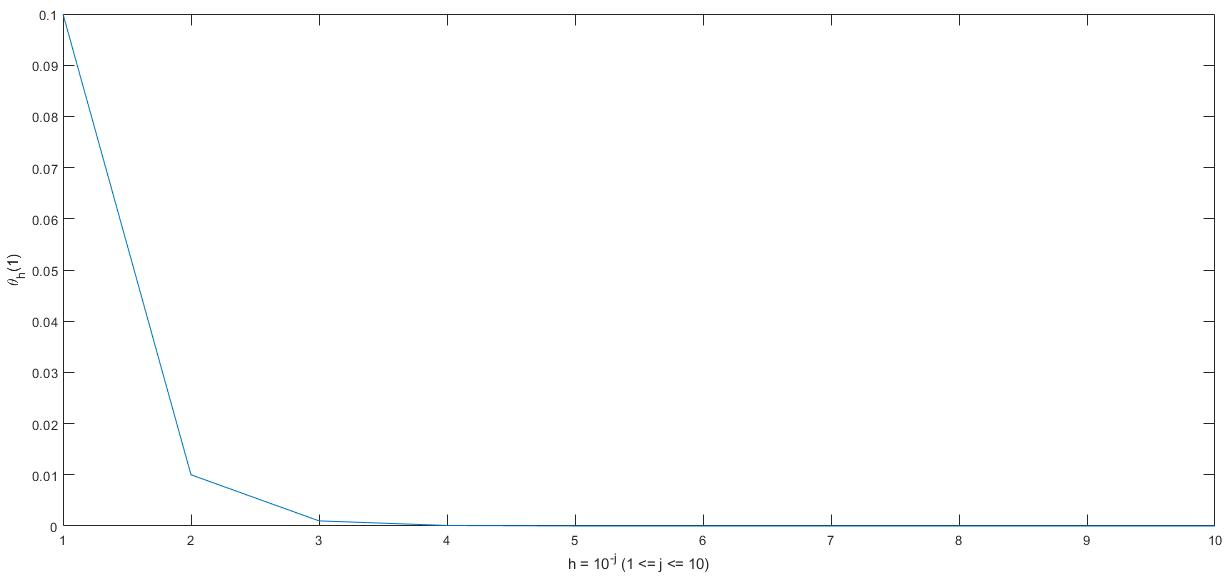
\includegraphics[width=\textwidth]{Plot/Cap_1_Es_3}
		\caption{Andamento della funzione $\theta_{h}(1)$}
\end{figure}
\subsection{Esercizio 4}
Le due espressioni in aritmetica finita vengono scritte tenendo conto dell'errore di approssimazione sul valore reale:\\
\begin{enumerate}
	\item $(x \oplus y) \oplus z \equiv fl(fl(fl(x)+fl(y))+fl(z)) = ((x(1+\varepsilon_{x})+y(1+\varepsilon_{y}))(1+\varepsilon_{a})+z(1+\varepsilon_{z}))(1+\varepsilon_{b})$
	\item $x \oplus (y \oplus z) \equiv fl(fl(x)+fl(fl(y)+fl(z))) = (x(1+\varepsilon_{x})+(y(1+\varepsilon_{y})+z(1+\varepsilon_{z}))(1+\varepsilon_{a}))(1+\varepsilon_{b})$\\
\end{enumerate}
Indichiamo con $\varepsilon_{x},\varepsilon_{y},\varepsilon_{z}$ i relativi errori di $x, y, z$ e con $\varepsilon_{a},\varepsilon_{b}$ gli errori delle somme e per calcolare l'errore relativo delle due espressioni consideriamo $\varepsilon_{m} = max\{|\varepsilon_{x}|,|\varepsilon_{y}|,|\varepsilon_{z}|,|\varepsilon_{a}|,|\varepsilon_{b}|\}$.\\
Dalla definizione di errore relativo si ha quindi:\\
\begin{enumerate}
    \item 
   		\[
    		\varepsilon_{1} = \frac{((x(1+\varepsilon_{x})+y(1+\varepsilon_{y}))(1+\varepsilon_{a})+z(1+\varepsilon_{z}))(1+\varepsilon_{b})-(x+y+z)}{x+y+z} \approx
    	\]
    	\[
    		\approx \frac{x(1+\varepsilon_{x}+\varepsilon_{a}+\varepsilon_{b})+y(1+\varepsilon_{y}+\varepsilon_{a}+\varepsilon_{b})+z(1+\varepsilon_{z}+\varepsilon_{b})-x-y-z}{x+y+z} \leq
    	\]
    	\[ 
    		\leq\left|\frac{\varepsilon_{b}(x+y+z)+\varepsilon_{a}(x+y)+x\varepsilon_{x}+y\varepsilon_{y}+z\varepsilon_{z}}{(x+y+z)}\right|\leq
    	\]
    	\[
    		\leq\frac{|\varepsilon_{b}||x+y+z|+|\varepsilon_{a}||x+y|+|x||\varepsilon_{x}|+|y||\varepsilon_{y}|+|z||\varepsilon_{z}|}{|x+y+z|}\leq
    	\]
    	\[
    		\leq\varepsilon_{m}\frac{|x+y+z|+|x+y|+(|x|+|y|+|z|)}{|x+y+z|}=
    	\]
    	\[
    		=\varepsilon_{m}\left(1+\frac{|x+y|}{|x+y+z|}+\frac{|x|+|y|+|z|}{|x+y+z|}\right)
    	\]\\\
    \item Tenendo presente che $x \oplus (y \oplus z) = (y \oplus z) \oplus x$, seguendo gli stessi procedimenti del punto precedente possiamo scrivere:\\
    	\[
    		\varepsilon_{2} = \frac{((y(1+\varepsilon_{y})+z(1+\varepsilon_{z}))(1+\varepsilon_{a})+x(1+\varepsilon_{x}))(1+\varepsilon_{b})-(y+z+x)}{y+z+x} \approx
    	\]
    	\[
    		\approx \frac{y(1+\varepsilon_{y}+\varepsilon_{a}+\varepsilon_{b})+z(1+\varepsilon_{z}+\varepsilon_{a}+\varepsilon_{b})+x(1+\varepsilon_{x}+\varepsilon_{b})-y-z-x}{y+z+x} \leq
    	\]
    	\[ 
    		\leq\left|\frac{\varepsilon_{b}(y+z+x)+\varepsilon_{a}(y+z)+y\varepsilon_{y}+z\varepsilon_{z}+x\varepsilon_{x}}{(y+z+x)}\right|\leq
    	\]
    	\[
    		\leq\frac{|\varepsilon_{b}||y+z+x|+|\varepsilon_{a}||y+z|+|y||\varepsilon_{y}|+|z||\varepsilon_{z}|+|x||\varepsilon_{x}|}{|y+z+x|}\leq
    	\]
    	\[
    		\leq\varepsilon_{m}\frac{|y+z+x|+|y+z|+(|y|+|z|+|x|)}{|y+z+x|}=
    	\]
    	\[
    		=\varepsilon_{m}\left(1+\frac{|y+z|}{|y+z+x|}+\frac{|y|+|z|+|x|}{|y+z+x|}\right)
    	\]\\\
\end{enumerate}
Otteniamo quindi che i valori degli errori $\varepsilon_{1}$ e $\varepsilon_{2}$ sono condizionati rispettivamente, dai valori $\frac{|x+y|}{|x+y+z|}$ e $\frac{|y+z|}{|y+z+x|}$.
\subsection{Esercizio 5}
Il seguente codice MatLab:\\
\lstinputlisting[language=Matlab]{Cap_1/Es_5/Es_5.m}
restituisce i seguenti valori:\\
\begin{enumerate}
\item $delta = 1/16$\\
Il valore di $delta=[0.0625]_{10}$ in binario si scrive $delta=[0,0001]_2$ . Al passo 16, che sarà il valore di \textit{count} la rappresentazione di $x$ sarà uguale a 1, e siccome l'unica condizione di uscita dello while è $x~=1$, il ciclo si arresterà.
\\
\item $delta = 1/20$\\
Il valore di $delta=[0,05]_{10}$ in binario si scrive $delta=[0,00\overline{0011}]_2$ . A differenza del caso precedente, si può notare che la rappresentazione del valore di delta in binario è periodica. Al passo 10 la rappresentazione di $x$ sarà diversa da 1, poichè la somma riguarda numeri periodici, e siccome l'unica condizione di uscita dello while è $x~=1$, il ciclo non si arresterà mai.\\
Possiamo provarlo effettuando la somma in binario di:
\[
\Big[\frac{1}{20}\Big]_{10}=\Big[0,00\overline{0011}\Big]_2
\]
\[
\Big[0,00\overline{0011}\Big]_2+\Big[0,00\overline{0011}\Big]_2+ \underbrace{...}_{6 volte}+\Big[0,00\overline{0011}\Big]_2+\Big[0,00\overline{0011}\Big]_2 = 
\]
\[
= [0.100011]_2 \approx [0.546875]_{10} \neq [1.00000]_{10}
\]
che spiegherebbe il motivo del loop dello while.
\end{enumerate}
\subsection{Esercizio 6}
\begin{enumerate}
	\item
		Il seguente codice MatLab, riguarda la prima successione $x_{k+1} = (x_k + 3/x_k)/2$, indicando con $x=x_k$, $r=\epsilon$ e $conv = \sqrt{3} \approx 1.73205080756888e+000$ :\\
		\lstinputlisting[language=Matlab]{Cap_1/Es_6/FirstSucc.m}
		restituisce i seguenti valori:\\
		\begin{center}
			\begin{tabular}{|c|c|c|}
			\hline
				$k$ & $x_k$ & $\epsilon_k$ \\
			\hline
    			$k=0$ & $x_0 = 3.00000000000000e+000$ & $\epsilon_0 = 1.26794919243112e+000$\\
    			$k=1$ & $x_1 = 2.00000000000000e+000$ & $\epsilon_1 =  267.949192431123e-003$\\
    			$k=2$ & $x_2 = 1.75000000000000e+000$ & $\epsilon_2 = 17.9491924311228e-003$\\
    			$k=3$ & $x_3 = 1.73214285714286e+000$ & $\epsilon_3 = 92.0495739800131e-006$\\
    			$k=4$ & $x_4 = 1.73205081001473e+000$ & $\epsilon_4 = 2.44585018904786e-009$\\
    			$k=5$ & $x_5 = 1.73205080756888e+000$ & $\epsilon_5 = 0.00000000000000e+000$\\
			\hline
			\end{tabular}
		\end{center}
		I calcoli indicano che per valori di $k$ superiori a 4, l'errore assoluto indicato con $\epsilon$, è dell'ordine di \(10^{-9}\), cioè $\leq$ \(10^{-12}\).\\
	\item
		Il seguente codice MatLab, riguarda la seconda successione $x_{k+1} = (3+x_{k-1}x_k)/(x_{k-1}x_k)$, indicando con $x=x_k$, $r=\epsilon$ e $conv = \sqrt{3} \approx 1.73205080756888e+000$ :\\
		\lstinputlisting[language=Matlab]{Cap_1/Es_6/SecondSucc.m}
		restituisce i valori:\\
		\begin{center}
			\begin{tabular}{|c|c|c|}
			\hline
				$k$ & $x_k$ & $\epsilon_k$ \\
			\hline
    			$k=0$ & $x_0 = 3.00000000000000e+000$ & $\epsilon_0 = 1.26794919243112e+000$\\
    			$k=1$ & $x_1 = 2.00000000000000e+000$ & $\epsilon_1 = 267.949192431123e-003$\\
    			$k=2$ & $x_2 = 1.80000000000000e+000$ & $\epsilon_2 = 67.9491924311229e-003$\\
    			$k=3$ & $x_3 = 1.73684210526316e+000$ & $\epsilon_3 = 4.79129769428077e-003$\\
    			$k=4$ & $x_4 = 1.73214285714286e+000$ & $\epsilon_4 = 92.0495739797911e-006$\\
    			$k=5$ & $x_5 = 1.73205093470604e+000$ & $\epsilon_5 = 127.137164351865e-009$\\
    			$k=6$ & $x_6 = 1.73205080757226e+000$ & $\epsilon_6 = 3.37863070853928e-012$\\
    			$k=7$ & $x_7 = 1.73205080756888e+000$ & $\epsilon_7 = 222.044604925031e-018$\\
			\hline
			\end{tabular}
		\end{center}
		I calcoli indicano che per valori di $k$ superiori a 6 incluso, l'errore assoluto indicato con $\epsilon$, è dell'ordine di \(10^{-12}\), cioè $\leq$ \(10^{-12}\).\\
\end{enumerate}
\newpage
\section{\textbf{Capitolo 2}}
\subsection{Esercizio 1}
Studio analitico del polinomio $P(x) = x^3-4x^2+5x-2$.\\
\begin{itemize}
	\item \textbf{Zeri del polinomio}\\
		Prima di tutto si scompone il polinomio :
			\[
			\ x^3-4x^2+5x-2 =
			\] 
			\[
			\ = x^3-2x^2+x-2-2x^2+4x =
			\]
			\[
			\ = x(x^2-2x+1)+2(1+x^2-2x) =
			\]
			\[
			\ = (x^2-2x+1)(x-2) =
			\]
			\[
			\ = (x-1)^2(x-2) 
			\]\\
		Quindi il polinomio si annulla $P(x)=0$ per $(x-1)=0 \Rightarrow x=1$ e $(x-2)=0 \Rightarrow x=2$. \\
	\item \textbf{Molteplicità}\\
		I valori di \textit{x} precedentemente calcolati vengono definiti come \textit{radici} del polinomio. Si dice che \textit{a} è una radice di \textit{P(x)} con \textit{molteplicità n} se e solo se \textit{P(x)} è divisibile per $(x-a)^n$, ma non è divisibile per $(x-a)^{n-1}$.\\
		Inoltre si dice che \textit{x} ha \textit{molteplicità esatta} $n \geq 1$, se:
			\[
			f(x) = f'(x) = ... = f^{(n-1)}(x) = 0,  f^{(n)}(x) \neq 0.
			\]
			\begin{itemize}
				\item $x=1$
					\[
					P(1) = 1-4+5-2 = 0 
					\]
					\[
					P'(1) = 3x^2-8x+5 = 3-8+5 = 0 
					\]
					\[
					P''(1) = 6x-8 = 6-8 \neq 0 \Rightarrow \textit{ molteplicità } n=2
					\]\\
				\item $x=2$
					\[
					P(2) = 8-16+10-2 = 0 
					\]
					\[
					P'(2) = 3x^2-8x+5 = 12-16+5 = 1 \neq 0 \Rightarrow \textit{ molteplicità } n=1
					\]
			\end{itemize}
		Quindi è che con $x=1$, la radice viene definita \textit{multipla} in quanto il polinomio viene annullato 2 volte, con molteplicità $n=2$; invece con $x=2$, la radice viene definita \textit{semplice} in quanto il polinomio viene annullato 1 volta,  con molteplicità $n=1$.\\ 
\end{itemize}
Il \textbf{metodo di bisezione} è utilizzabile per approssimarne uno delle due radice a partire dall'intervallo di confidenza \textit{[a,b]=[0,3]} se e solo se il polinomio dato $P(x)=0$ definito e continuo nell'intervallo di confidenza \textit{[a,b]=[0,3]}, tale che $P(a)*P(b) < 0$, è allora possibile calcolarne un'approssimazione in \textit{[a,b]}.\\\\
	\[
	P(a) = P(0) = -2
	\]
	\[
	P(b) = P(3) = 4
	\]
	\[
	P(a)*P(b) = -2 * 4 = -8 < 0
	\]\\
Essendo il polinomio continuo, le ipotesi sono rispettate. Infatti entrambe le radici $x \in \{1,2\}$, appartengono all'intervallo di confidenza \textit{[a,b]=[0,3]}.\\\\
Il seguente codice MatLab, riguarda il \textbf{Metodo di bisezione}:\\
	\lstinputlisting[language=Matlab]{Cap_2/Es_1/bisezione.m}
Il seguente codice MatLab, riguarda il polinomio $P(x) = x^3-4x^2+5x-2$, su quale viene eseguito il metodo di bisezione, con intervallo di confidenza \textit{[a,b]=[0,3]} e valore di $tol_x=10^{-1}$ che decresce ad ogni passaggio:\\
	\lstinputlisting[language=Matlab]{Cap_2/Es_1/Es_1.m}
restituisce i seguenti valori:\\
\begin{center}
	\begin{tabular}{|c|c|c|}
		\hline
			$tol_x$ & \textit{Bisezione} & \textit{Num. Iterazioni} \\
		\hline
   			$10^{-1}$ & $\tilde{x} = 1.5000$ & $ib = 0$\\
    		$10^{-2}$ & $\tilde{x} = 1.9922$ & $ib = 6$\\
    		$10^{-3}$ & $\tilde{x} = 2.0010$ & $ib = 9$\\
    		$10^{-4}$ & $\tilde{x} = 2.0001$ & $ib = 13$\\
   			$10^{-5}$ & $\tilde{x} = 2.0000$ & $ib = 16$\\
   			$10^{-6}$ & $\tilde{x} = 2.0000$ & $ib = 19$\\
    		$10^{-7}$ & $\tilde{x} = 2.0000$ & $ib = 23$\\
    		$10^{-8}$ & $\tilde{x} = 2.0000$ & $ib = 26$\\
    		$10^{-9}$ & $\tilde{x} = 2.0000$ & $ib= 29$\\
    		$10^{-10}$ & $\tilde{x} = 2.0000$ & $ib = 33$\\
    		$10^{-11}$ & $\tilde{x} = 2.0000$ & $ib = 36$\\
    		$10^{-12}$ & $\tilde{x} = 2.0000$ & $ib = 39$\\
    		$10^{-13}$ & $\tilde{x} = 2.0000$ & $ib = 43$\\
    		$10^{-14}$ & $\tilde{x} = 2.0000$ & $ib = 46$\\
    		$10^{-15}$ & $\tilde{x} = 2.0000$ & $ib = 49$\\
		\hline
	\end{tabular}
\end{center}
\subsection{Esercizio 2}
Abbiamo visto come il polinomio $P(x) = x^3-4x^2+5x-2$, in $P(x)=0$ presenta due radici, una con molteplicità multipla $x=1$ e una con molteplicità semplice $x=2$.\\\\
Di seguito sono riportati tre codici MatLab, rispettivamente:
\begin{itemize}
	\item \textbf{Metodo di Newton}
		\lstinputlisting[language=Matlab]{Cap_2/Es_2/newton.m}
	\item \textbf{Metodo delle Corde}
		\lstinputlisting[language=Matlab]{Cap_2/Es_2/corde.m}
	\item \textbf{Metodo delle Secanti}
		\lstinputlisting[language=Matlab]{Cap_2/Es_2/secanti.m}
\end{itemize}
Il seguente codice MatLab, riguarda il polinomio $P(x) = x^3-4x^2+5x-2$, sul quale vengono eseguiti il metodo di Newton, il metodo delle Corde e il metodo delle Secanti (con secondo termine della successione ottenuto con Newton), valore di $tol_x=10^{-1}$ che decresce ad ogni passaggio, \textit{pd} che indica la derivata del polinomio, numero di iterazioni massime 1000 e punto di partenza $x_{0}=3$:\\
	\lstinputlisting[language=Matlab]{Cap_2/Es_2/Es_2.m}
restituisce i seguenti valori:\\
\begin{center}
	\begin{tabular}{|c|c|c|c|}
		\hline
			$tol_x$ & \textit{Newton} & \textit{Corde} & \textit{Secanti} \\
		\hline
			$10^{-1}$ & $\tilde{x}$ = 2.0043 \quad \textit{i} = 4 & $\tilde{x}$ = 2.2764 \quad \textit{i} = 3 & $\tilde{x}$ = 2.1375 \quad \textit{i} = 4\\
			$10^{-2}$ & $\tilde{x}$ = 2.0000 \quad \textit{i} = 5 & $\tilde{x}$ = 2.0552 \quad \textit{i} = 12 & $\tilde{x}$ = 2.1375 \quad \textit{i} = 6\\
			$10^{-3}$ & $\tilde{x}$ = 2.0000 \quad \textit{i} = 6 & $\tilde{x}$ = 2.0067 \quad \textit{i} = 27 & $\tilde{x}$ = 2.0010 \quad \textit{i} = 7\\
			$10^{-4}$ & $\tilde{x}$ = 2.0000 \quad \textit{i} = 6 & $\tilde{x}$ = 2.0001 \quad \textit{i} = 44 & $\tilde{x}$ = 2.0000 \quad \textit{i} = 8\\
			$10^{-5}$ & $\tilde{x}$ = 2.0000 \quad \textit{i} = 7 & $\tilde{x}$ = 2.0000 \quad \textit{i} = 62 & $\tilde{x}$ = 2.0000 \quad \textit{i} = 9\\
			$10^{-6}$ & $\tilde{x}$ = 2.0000 \quad \textit{i} = 7 & $\tilde{x}$ = 2.0000 \quad \textit{i} = 79 & $\tilde{x}$ = 2.0000 \quad \textit{i} = 9\\
			$10^{-7}$ & $\tilde{x}$ = 2.0000 \quad \textit{i} = 7 & $\tilde{x}$ = 2.0000 \quad \textit{i} = 96 & $\tilde{x}$ = 2.0000 \quad \textit{i} = 9\\
			$10^{-8}$ & $\tilde{x}$ = 2.0000 \quad \textit{i} = 7 & $\tilde{x}$ = 2.0000 \quad \textit{i} = 113 & $\tilde{x}$ = 2.0000 \quad \textit{i} = 10\\
			$10^{-9}$ & $\tilde{x}$ = 2.0000 \quad \textit{i} = 8 & $\tilde{x}$ = 2.0000 \quad \textit{i} = 131 & $\tilde{x}$ = 2.0000 \quad \textit{i} = 10\\
			$10^{-10}$ & $\tilde{x}$ = 2.0000 \quad \textit{i} = 8 & $\tilde{x}$ = 2.0000 \quad \textit{i} = 148 & $\tilde{x}$ = 2.0000 \quad \textit{i} = 10\\
			$10^{-11}$ & $\tilde{x}$ = 2.0000 \quad \textit{i} = 8 & $\tilde{x}$ = 2.0000 \quad \textit{i} = 165 & $\tilde{x}$ = 2.0000 \quad \textit{i} = 10\\
			$10^{-12}$ & $\tilde{x}$ = 2.0000 \quad \textit{i} = 8 & $\tilde{x}$ = 2.0000 \quad \textit{i} = 182 & $\tilde{x}$ = 2.0000 \quad \textit{i} = 11\\
			$10^{-13}$ & $\tilde{x}$ = 2.0000 \quad \textit{i} = 8 & $\tilde{x}$ = 2.0000 \quad \textit{i} = 199 & $\tilde{x}$ = 2.0000 \quad \textit{i} = 11\\
			$10^{-14}$ & $\tilde{x}$ = 2.0000 \quad \textit{i} = 8 & $\tilde{x}$ = 2.0000 \quad \textit{i} = 217 & $\tilde{x}$ = 2.0000 \quad \textit{i} = 11\\
			$10^{-15}$ & $\tilde{x}$ = 2.0000 \quad \textit{i} = 8 & $\tilde{x}$ = 2.0000 \quad \textit{i} = 233 & $\tilde{x}$ = 2.0000 \quad \textit{i} = 11\\
		\hline
	\end{tabular}
\end{center}
Si vede da questi risultati che i metodi di Newton e delle Secanti convergono molto velocemente alla soluzione, mentre il metodo delle Corde, seppur convergendo, richiede molti più passi d'iterazione. Tuttavia, osservando il tempo d'esecuzione impiegato dai tre metodi per eseguire un singolo step, si deduce che i metodi quasi-Newton (Corde e Secanti) hanno un tempo di esecuzione medio per step inferiore a quello del metodo di Newton: infatti, in media, un passo d'iterazione del metodo delle secanti dura circa $\frac{1}{2}$ rispetto a quello di Newton e quello delle corde $\frac{1}{4}$. Quindi, in questo caso, il metodo più efficiente sembra essere quello delle secanti, che combina un'alta convergenza con un basso tempo di esecuzione.\\\\
La scelta del \textbf{valore di innesco} $x_{0}$ è importante. Un metodo \textit{converge localmente} ad $\alpha$ se la convergenza della successione dipende in modo critico dalla vicinanza di $x_{0}$ ad $\alpha$. Il procedimento è \textit{globalmente convergente} quando la convergenza non dipende da quanto $x_{0}$ è vicino ad $\alpha$. Per i metodi a convergenza locale la scelta del punto di innesco è cruciale.\\
E' possibile utilizzare $x_{0}=5/3$ come punto di innesco, in quanto essendo tutti e tre i metodi (\textbf{Newton, Corde e Secanti}) localmente convergenti, più la differenza con la radice è minore più velocemente converge. Infatti:
	\[
	|alpha_1 - x_{0}| = |2 - 5/3| = 0,\overline{3} \leq 1 = |2 - 3| = |alpha_1 - x|
	\]
	\[
	|alpha_2 - x_{0}| = |1 - 5/3| = 0,\overline{6} \leq 2 = |1 - 3| = |alpha_2 - x|
	\]
\subsection{Esercizio 3}
Abbiamo visto come il polinomio $P(x) = x^3-4x^2+5x-2$, in $P(x)=0$ presenta due radici, una con molteplicità multipla $x=1$ e una con molteplicità semplice $x=2$.\\\\
Di seguito sono riportati tre codici MatLab, rispettivamente:
\begin{itemize}
	\item \textbf{Metodo di Newton}
		\lstinputlisting[language=Matlab]{Cap_2/Es_2/newton.m}
	\item \textbf{Metodo di Newton modificato}
		\lstinputlisting[language=Matlab]{Cap_2/Es_3/newtonMod.m}
	\item \textbf{Metodo di Aitken}
		\lstinputlisting[language=Matlab]{Cap_2/Es_3/aitken.m}
\end{itemize}
Il seguente codice MatLab, riguarda il polinomio $P(x) = x^3-4x^2+5x-2$, sul quale vengono eseguiti il metodo di Newton, il metodo di Newton modificato (con molteplicità $m=1$ per la radice $x=2$ e $m=2$ per la radice $x=1$) e il metodo di Aitken, valore di $tol_x=10^{-1}$ che decresce ad ogni passaggio, \textit{pd} che indica la derivata del polinomio, numero di iterazioni massime 1000 e punto di partenza $x_{0}=0$:\\
	\lstinputlisting[language=Matlab]{Cap_2/Es_3/Es_3.m}
restituisce i seguenti valori:\\
\begin{center}
	\begin{tabular}{|c|c|c|c|c|}
		\hline
			$tol_x$ & \textit{Newton} & \textit{NewtonMod $m=1$} & \textit{NewtonMod $m=2$} & \textit{Aitken} \\
		\hline
			$10^{-1}$ & $\tilde{x} = 0.8960$ \quad $in = 4$ & $\tilde{x} = 0.8960$ \quad $inm_1 = 4$ & $\tilde{x} = 0.9999$ \quad $inm_2 = 3$ & $\tilde{x} = 1.0020$ \quad $ia = 2$\\
			$10^{-2}$ & $\tilde{x} = 0.9929$ \quad $in = 8$ & $\tilde{x} = 0.9929$ \quad $inm_1 = 8$ & $\tilde{x} = 1.0000$ \quad $inm_2 = 4$ & $\tilde{x} = 1.0000$ \quad $ia = 3$\\
			$10^{-3}$ & $\tilde{x} = 0.9991$ \quad $in = 11$ & $\tilde{x} = 0.9991$ \quad $inm_1 = 11$ & $\tilde{x} = 1.0000$ \quad $inm_2 = 4$ & $\tilde{x} = 1.0000$ \quad $ia = 4$\\
			$10^{-4}$ & $\tilde{x} = 0.9999$ \quad $in = 15$ & $\tilde{x} = 0.9999$ \quad $inm_1 = 15$ & $\tilde{x} = 1.0000$ \quad $inm_2 = 5$ & $\tilde{x} = 1.0000$ \quad $ia = 4$\\
			$10^{-5}$ & $\tilde{x} = 1.0000$ \quad $in = 18$ & $\tilde{x} = 1.0000$ \quad $inm_1 = 18$ & $\tilde{x} = 1.0000$ \quad $inm_2 = 5$ & $\tilde{x} = 1.0000$ \quad $ia = 4$\\
			$10^{-6}$ & $\tilde{x} = 1.0000$ \quad $in = 21$ & $\tilde{x} = 1.0000$ \quad $inm_1 = 21$ & $\tilde{x} = 1.0000$ \quad $inm_2 = 5$ & $\tilde{x} = 1.0000$ \quad $ia = 4$\\
			$10^{-7}$ & $\tilde{x} = 1.0000$ \quad $in = 25$ & $\tilde{x} = 1.0000$ \quad $inm_1 = 25$ & $\tilde{x} = 1.0000$ \quad $inm_2 = 5$ & $\tilde{x} = 1.0000$ \quad $ia = 4$\\
			$10^{-8}$ & $\tilde{x} = 1.0000$ \quad $in = 29$ & $\tilde{x} = 1.0000$ \quad $inm_1 = 29$ & $\tilde{x} = 1.0000$ \quad $inm_2 = 5$ & $\tilde{x} = 1.0000$ \quad $ia = 4$\\
			$10^{-9}$ & $\tilde{x} = 1.0000$ \quad $in = 29$ & $\tilde{x} = 1.0000$ \quad $inm_1 = 29$ & $\tilde{x} = 1.0000$ \quad $inm_2 = 5$ & $\tilde{x} = 1.0000$ \quad $ia = 4$\\
			$10^{-10}$ & $\tilde{x} = 1.0000$ \quad $in = 29$ & $\tilde{x} = 1.0000$ \quad $inm_1 = 29$ & $\tilde{x} = 1.0000$ \quad $inm_2 = 5$ & $\tilde{x} = 1.0000$ \quad $ia = 4$\\
			$10^{-11}$ & $\tilde{x} = 1.0000$ \quad $in = 29$ & $\tilde{x} = 1.0000$ \quad $inm_1 = 29$ & $\tilde{x} = 1.0000$ \quad $inm_2 = 5$ & $\tilde{x} = 1.0000$ \quad $ia = 4$\\
			$10^{-12}$ & $\tilde{x} = 1.0000$ \quad $in = 29$ & $\tilde{x} = 1.0000$ \quad $inm_1 = 29$ & $\tilde{x} = 1.0000$ \quad $inm_2 = 5$ & $\tilde{x} = 1.0000$ \quad $ia = 4$\\
			$10^{-13}$ & $\tilde{x} = 1.0000$ \quad $in = 29$ & $\tilde{x} = 1.0000$ \quad $inm_1 = 29$ & $\tilde{x} = 1.0000$ \quad $inm_2 = 5$ & $\tilde{x} = 1.0000$ \quad $ia = 4$\\
			$10^{-14}$ & $\tilde{x} = 1.0000$ \quad $in = 29$ & $\tilde{x} = 1.0000$ \quad $inm_1 = 29$ & $\tilde{x} = 1.0000$ \quad $inm_2 = 5$ & $\tilde{x} = 1.0000$ \quad $ia = 4$\\
			$10^{-15}$ & $\tilde{x} = 1.0000$ \quad $in = 29$ & $\tilde{x} = 1.0000$ \quad $inm_1 = 29$ & $\tilde{x} = 1.0000$ \quad $inm_2 = 5$ & $\tilde{x} = 1.0000$ \quad $ia = 4$\\
		\hline
	\end{tabular}
\end{center}
Si vede da questi risultati che i metodi di Newton modificato con molteplicità $m=2$ e di Aitken convergono molto velocemente alla soluzione, mentre il metodo di Newton e di Newton modificato con $m=1$ (tale valore di molteplicità rende identici i valori restituiti), seppur convergendo, richiedono più passi d'iterazione.
\subsection{Esercizio 4}
Essendo $\sqrt{\alpha}$ la radice ricercata, dobbiamo innanzitutto trovare una funzione $f(x)$ che abbia uno zero in $x=\sqrt{\alpha}$. La funzione più semplice di questo tipo è $f(x)=x-\sqrt{\alpha}$, ma ovviamente, dato che si sta tentando di approssimare $\sqrt{\alpha}$ stessa, non è verosimile utilizzare il valore esatto per il calcolo dell'approssimazione. Quindi si
utilizza la funzione $f(x) = x^2-\alpha$, che ha radici semplici in $x=\sqrt{\alpha}$ e in $x=-\sqrt{\alpha}$, ovvero $f(\pm\sqrt{\alpha})=0$. La derivata prima di questa funzione è $f'(x)=2x$.\\\\
L'iterazione del metodo di Newton utilizzando questa funzione diventa :
	\[
	x_{i+1} = x_i-\frac{f(x_i)}{f'(x_i)} = x_i - \frac{x_i^2-\alpha}{2x_i} =
	\]
	\[
	= \frac{2x_i^2-x_i^2+\alpha}{2x_i} = \frac{x_i^2+\alpha}{2x_i} =
	\]
	\[
	= \frac{1}{2} \Bigl( x_i+\frac{\alpha}{x_i} \Bigl),\quad i=0,1,2,...
	\]\\\\
Il seguente codice MatLab, riguarda l'implementazione del \textbf{metodo di Newton per il calcolo} $\sqrt{\alpha}$:\\ 
	\lstinputlisting[language=Matlab]{Cap_2/Es_4/newtonSqrtAlpha.m}
Il seguente codice MatLab, riguarda la chiamata della funzione definita precedentemente, con $\alpha=x_0=5$, con numero di passi massimi $imax=100$ e indice di tolleranza $tol_x=eps$ :\\
	\lstinputlisting[language=Matlab]{Cap_2/Es_4/Es_4.m}
restituisce i seguenti valori:\\
\begin{center}
	\begin{tabular}{|c|c|c|}
		\hline
			$i$ & $x_i$ & $E_{ass}=\epsilon_i=|x_i-\sqrt{\alpha}| \quad \alpha=5$ \\
		\hline
    		$i=0$ & $x_0 = 5$ & $|\epsilon_0| = 2.763932022500210e+00$\\
    		$i=1$ & $x_1 = 3$ & $|\epsilon_1| = 7.639320225002102e-01$\\
    		$i=2$ & $x_2 = 2.333333333333333e+00$ & $|\epsilon_2| = 9.726535583354368e-02$\\
    		$i=3$ & $x_3 = 2.238095238095238e+00$ & $|\epsilon_3| = 2.027260595448332e-03$\\
    		$i=4$ & $x_4 = 2.236068895643363e+00$ & $|\epsilon_4| = 9.181435736138610e-07$\\
    		$i=5$ & $x_5 = 2.236067977499978e+00$ & $|\epsilon_5| = 1.882938249764265e-13$\\
    		$i=6$ & $x_6 = 2.236067977499790e+00$ & $|\epsilon_6| = 0$\\
    		$i=7$ & $x_7 = 2.236067977499790e+00$ & $|\epsilon_7| = 0$\\
		\hline
	\end{tabular}
\end{center}
\subsection{Esercizio 5}
Come precedentemente visto nell'Esercizio 2.4 si utilizzerà la funzione $f(x) = x^2-\alpha$, che ha radici semplici in $x=\sqrt{\alpha}$ e in $x=-\sqrt{\alpha}$, ovvero $f(\pm\sqrt{\alpha})=0$. La derivata prima di questa funzione è $f'(x)=2x$.\\\\
L'iterazione del metodo delle Secanti utilizzando questa funzione diventa :
	\[
	x_{i+1} = \frac{f(x_i)x_{i-1}-f(x_{i-1})x_i}{f(x_i)-f(x_{i-1})} =
	\]
	\[
	= \frac{(x_i^2-\alpha)x_{i-1}-(x_{i-1}^2-\alpha)x_i}{x_i^2-\alpha-x_{i-1}^2+\alpha}  =
	\]
	\[
	= \frac{x_i^2x_{i-1}-\alpha x_{i-1}-x_{i-1}^2x_i+\alpha x_i}{x_i^2-x_{i-1}^2} =
	\]
	\[
	= \frac{x_ix_{i-1}(x_i-x_{i-1})+\alpha (x_i-x_{i-1})}{(x_i-x_{i-1})(x_i+x_{i-1})} =
	\]
	\[
	= \frac{(x_i-x_{i-1})(x_ix_{i-1}+\alpha)}{(x_i-x_{i-1})(x_i+x_{i-1})} =
	\]
	\[
	= \frac{x_ix_{i-1}+\alpha}{x_i+x_{i-1}},\quad i=0,1,2,...
	\]\\\\
Il seguente codice MatLab, riguarda l'implementazione del \textbf{metodo delle Secanti per il calcolo} $\sqrt{\alpha}$:\\ 
	\lstinputlisting[language=Matlab]{Cap_2/Es_5/secantiSqrtAlpha.m}
Il seguente codice MatLab, riguarda la chiamata della funzione definita precedentemente, con $\alpha=x_0=5$, con $x_1=3$, con numero di passi massimi $imax=100$ e indice di tolleranza $tol_x=eps$ :\\
	\lstinputlisting[language=Matlab]{Cap_2/Es_5/Es_5.m}
restituisce i seguenti valori:\\
\begin{center}
	\begin{tabular}{|c|c|c|}
		\hline
			$i$ & $x_i=xs$ & $E_{ass}=exs=\epsilon_i=|x_i-\sqrt{\alpha}| \quad \alpha=5$ \\
		\hline
    		0 & $x_0$ = 5 & $|\epsilon_0|$ = 2.763932022500210e+00\\
    		1 & $x_1$ = 3 & $|\epsilon_1|$ = 7.639320225002102e-01\\
    		2 & $x_2$ = 2.500000000000000e+00 & $|\epsilon_2|$ = 2.639320225002102e-01\\
    		3 & $x_3$ = 2.272727272727273e+00 & $|\epsilon_3|$ = 3.665929522748312e-02\\
    		4 & $x_4$ = 2.238095238095238e+00 & $|\epsilon_4|$ = 2.027260595448332e-03\\
    		5 & $x_5$ = 2.236084452975048e+00 & $|\epsilon_5|$ = 1.647547525829296e-05\\
    		6 & $x_6$ = 2.236067984964863e+00 & $|\epsilon_6|$ = 7.465073448287285e-09\\
    		7 & $x_7$ = 2.236067977499817e+00 & $|\epsilon_7|$ = 2.753353101070388e-14\\
    		8 & $x_8$ = 2.236067977499790e+00 & $|\epsilon_8|$ = 4.440892098500626e-16\\
    		9 & $x_9$ = 2.236067977499790e+00 & $|\epsilon_9|$ = 0\\
    		10 & $x_{10}$ = 2.236067977499790e+00 & $|\epsilon_{10}|$ = 0\\
		\hline
	\end{tabular}
\end{center}
Si può notare come la \textit{convergenza superlineare} sia leggermente più lenta rispetto alla \textit{convergenza quadratica} del metodo di Newton visto nell'esercizio precedente (2.4).
\newpage
\section{\textbf{Capitolo 3}}
\subsection{Esercizio 1}
Il seguente codice MatLab, contiene l'implementazione di una funzione per la risoluzione di un sistema lineare con matrice triangolare inferiore :\\\
\lstinputlisting[language=Matlab]{Cap_3/Es_1/triangolareInferiore.m}
Il seguente codice MatLab, contiene la chiamata della funzione precedente:\\\
\lstinputlisting[language=Matlab]{Cap_3/Es_1/Es_1.m}
con i seguenti parametri di input :\\\
\[
A =\begin{bmatrix}
	1 & 2 & 0 \\ 
	2 & 1 & 0 \\
	2 & 2 & 1 
\end{bmatrix}
\]\\\	
\[
b =\begin{bmatrix}
  2 \\
  2 \\
  2
\end{bmatrix}
\]\\\
restituendo il seguente vettore :\\\
\[
x =\begin{bmatrix}
  2 \\
  -2 \\
  2
\end{bmatrix}
\]
\subsection{Esercizio 2}
\graphicspath{ {assets/cap3/es_2/} }

Il seguente codice MatLab, contiene l'implementazione di una funzione per la \textit{fattorizzazione} $LDL^t$ di una matrice \textit{A}\\\
\begin{itemize}
	\item \textbf{Metodo fattorizzazione $LDL^t$}
	      \lstinputlisting[language=Matlab]{Cap_3/Es_2/fattorizzazioneLDLt.m}
\end{itemize}
Il seguente codice MatLab, contiene la chiamata della funzione precedente :\\\
\lstinputlisting[language=Matlab]{Cap_3/Es_2/Es_2.m}
con i seguenti parametri di input :\\\
\begin{enumerate}
	\item
	      \[
	      	A_1 =\begin{bmatrix}
	      	1  & -1  & 2   & 2  \\ 
	      	-1 & 5   & -14 & 2  \\
	      	2  & -14 & 42  & 2  \\
	      	2  & 2   & 2   & 65 
	      	\end{bmatrix}
	      \]\\
	\item
	      \[
	      	A_2 =\begin{bmatrix}
	      	1  & -1  & 2   & 2   \\ 
	      	-1 & 6   & -17 & 3   \\
	      	2  & -17 & 48  & -16 \\
	      	2  & 3   & -16 & 4   
	      	\end{bmatrix}
	      \]\\
\end{enumerate}
restituendo i seguenti risultati:\\\
\begin{enumerate}
	\item
	      $A_1$ è fattorizzabile $LDL^t$\\
	      \[
	      	LDL^t_1 =\begin{bmatrix}
	      	1  & -1  & 2   & 2  \\ 
	      	-1 & 4   & -14 & 2  \\
	      	2  & -3  & 2   & 2  \\
	      	2  & 1   & 5   & 7 
	      	\end{bmatrix}
	      \]
	      E' quindi \textit{sdp}.\\
	\item
	      $A_2$ non è fattorizzabile $LDL^t$, quindi non è \textit{sdp}. L'esecuzionde dell'$Es_2$ stamperà:\\\
	   	  \begin{center}
	   	  	\textit{Error using fattorizzazioneLDLt (line 23)}\\
	   	  	\textit{La matrice non è SDP}
	      \end{center}
\end{enumerate}
\subsection{Esercizio 3}
Per la risoluzione di un sistema lineare $Ax=b$ con $A=LDL^t$ , viene chiamato il seguente codice in MatLab:\\\
\begin{itemize}
\item \textbf{Metodo risoluzione $LDL^tx=b$}
\lstinputlisting[language=Matlab]{Cap_3/Es_3/risolutoreLDLt.m}
il quale implementa in ordine:
\begin{enumerate}
\item \textbf{fattorizzazioneLDLt($LDL^t$)}\\
Una funzione di fattorizzazione di un matrice $LDL^t$ passata come input e restituisce una matrice \textit{A} riscritta con le informazioni di \textit{L}, \textit{D} e $L^t$ (guarda es. 3.2).\\\
\item \textbf{triangolareInferiore(L,b)}\\
Una funzione per il calcolo del vettore incognite $x_1$ di una matrice triangolare inferiore a diagonale unitaria \textit{L} (con l'utilizzo dei comandi \textit{tril($LDL^t$,k<0)} che restituisce gli elementi sotto la k-esima diagonale di $LDL^t$; \textit{eye(n)} che restituisce una matrice di identità (tutti i valori zeri a parte i termini diagonali) di grandezza \textit{n}) passata come input insieme al vettore dei termini noti \textit{b} del sistema (guarda es. 3.1). \\\
\item \textbf{diagonale(D,$x_1$)}\\
Una funzione per il calcolo del vettore incognite $x_2$ di una matrice diagonale \textit{D} (con l'utilizzo del comando \textit{diag(A)} due volte, in quando la prima mi restituisce un vettore colonna degli elementi diagonali principali di $LDL^t$ e la seconda una matrice diagonale con tutti e solo gli elementi della diagonale $\neq 0$ ) passata come input insieme al vettore dei termini noti $x_1$:\\\
\begin{itemize}
\item \textbf{Metodo 'vettore' diagonale}
\lstinputlisting[language=Matlab]{Cap_3/Es_3/diagonale.m}
\end{itemize}
\item \textbf{triangolareSuperiore($L^t$,b)}\\
Una funzione per il calcolo del vettore incognite finale $x$ del sistema lineare di una matrice triangolare superiore a diagonale unitaria \textit{$L^t$} (con l'utilizzo dei comandi \textit{tril($LDL^t$,k<0)} che restituisce gli elementi sotto la k-esima diagonale di $LDL^t$; \textit{eye(n)} che restituisce una matrice di identità (tutti i valori zeri a parte i termini diagonali) di grandezza \textit{n}; al tutto viene aggiunta un \textit{apice " ' "} per calcolarne la trasposta) passata come input insieme al vettore dei termini noti $x_2$:\\\
\begin{itemize}
\item \textbf{Metodo matrice triangolare superiore}
\lstinputlisting[language=Matlab]{Cap_3/Es_3/triangolareSuperiore.m}
\end{itemize}
\end{enumerate}
\end{itemize}
\subsection{Esercizio 4}
Per la risoluzione di un sistema lineare $Ax=b$ con $A=LU$ , viene chiamato il seguente codice in MatLab:\\\
\begin{itemize}
	\item \textbf{Metodo risoluzione $LUx=b$ con pivoting}
		\lstinputlisting[language=Matlab]{Cap_3/Es_4/risolutoreLUpiv.m}
\end{itemize}
il quale implementa in ordine:
\begin{enumerate}
	\item \textbf{fattorizzazioneLUpiv(LU,b)}\\
		Una funzione di fattorizzazione di un matrice \textit{LU} passata come input che restituisce una matrice \textit{A} riscritta con le informazioni di \textit{L} e \textit{U} insieme a un vettore \textit{p} che indica le righe permutate :\\\
\begin{itemize}
	\item \textbf{Metodo fattorizzazione $LU$ con pivoting}
		\lstinputlisting[language=Matlab]{Cap_3/Es_4/fattorizzazioneLUpiv.m}
\end{itemize}
	\item \textbf{triangolareInferiore(L,b)}
		Una funzione per il calcolo del vettore incognite $x_1$ di una matrice triangolare inferiore a diagonale unitaria \textit{A} (con l'utilizzo dei comandi \textit{tril(A,k<0)} che restituisce gli elementi sotto la k-esima diagonale di A; \textit{eye(n)} che restituisce una matrice di identità (tutti i valori zeri a parte i termini diagonali) di grandezza \textit{n}) passata come input insieme al vettore dei termini noti \textit{b} del sistema, moltiplicato per la matrice di permutazione \textit{P} calcolata $P*b$ (guarda es. 3.3). \\\
	\item \textbf{triangolareSuperiore(U,b)}
		Una funzione per il calcolo del vettore incognite finale $x$ del sistema lineare di una matrice triangolare superiore a diagonale unitaria \textit{A} (con l'utilizzo dei comandi \textit{tril(A,k>0)} che restituisce gli elementi sopra la k-esima diagonale di A; \textit{eye(n)} che restituisce una matrice di identità (tutti i valori zeri a parte i termini diagonali) di grandezza \textit{n}) passata come input insieme al vettore dei termini noti $b=x_1$ (guarda es. 3.3).\\\
\end{enumerate}
\subsection{Esercizio 5}
Il seguente codice MatLab, contiene la chiamata delle due funzioni descritte negli esercizi precedenti, (\textit{risolutoreLDLt}  dell'es. 3.3 e risolutoreLUpiv dell'es. 3.4) per dimostrarne l'utilizzo tramite alcuni esempi:\\\
	\lstinputlisting[language=Matlab]{Cap_3/Es_5/Es_5.m}
\begin{description}
	\item \textbf{Esempio :} \textit{$risolutoreLDL^t$}\\\\
		con i seguenti parametri di input :\\\	 
		\[
		A_1 = LDL^t =\begin{bmatrix}
			3 & 2 & -1 \\ 
			2 & 7 &  7 \\
			-1 & 7 & 30 
		\end{bmatrix} \quad
		\hat{x_1} =\begin{bmatrix}
			4 \\
			5 \\
			3                
		\end{bmatrix} \quad
		b_1 = LDL^t \hat{x_1} =\begin{bmatrix}
			19 \\
			64 \\
			121                
		\end{bmatrix}
		\]\\
		\[
		L =\begin{bmatrix}
			1 		& 0 	 & 0 \\ 
			0,6667  & 1 	 & 0 \\
	   		-0,3333 & 1.3529 & 1 
		\end{bmatrix} \quad
		D =\begin{bmatrix}
			3 & 0      & 0 	     \\ 
			0 & 5.6667 & 0       \\
			0 & 0      & 19.2941 
		\end{bmatrix} \quad
		L^t =\begin{bmatrix}
			1 & 0.6667 & -0.3333 \\ 
			0 & 1      &  1.3529 \\
			0 & 0      &  1 
		\end{bmatrix}
		\]\\\\
	Il risultato ottenuto è:\\
		\[
		x_1 =\begin{bmatrix}
			4.00000000000000000 \\
			4.99999999999999999 \\
			3.00000000000000000                
		\end{bmatrix} \quad
		r_1 = LDL^t*x_1-b_1 =\begin{bmatrix}
			0 \\
		  	-7.1054e-15 \\
		  	0
		\end{bmatrix}
		\]\\\\
\item \textbf{Esempio :} \textit{risolutoreLUpiv}\\\\	
	con i seguenti parametri di input :\\\	  
		\[
		A_2 = LU =\begin{bmatrix}
			-23 & 5  & -21 & 8 \\ 
			0 	& 0  & 5   & 7 \\
			1 	& 54 & 7   & 9 \\
			0 	& -8 & 12  & 4  
		\end{bmatrix} \quad
		\hat{x_2} =\begin{bmatrix}
			2 \\
			8 \\
			3 \\
			5               
		\end{bmatrix} \quad
		b_2 = LDL^t \hat{x_2} =\begin{bmatrix}
			-29 \\
			50  \\
			500 \\
			-8                
		\end{bmatrix}
		\]\\
		\[
		L =\begin{bmatrix}
			1   	&  0  		& 0 	 & 0 \\ 
			-0.0435 &  1  		& 0 	 & 0 \\
		 	0   	&  -0.1476  & 1 	 & 0 \\
		 	0   	&  0  		& 0.3877 & 1 		    
		\end{bmatrix} \quad
		U =\begin{bmatrix}
			-23 & 5 	  & -21		& 8   	   \\ 
			0 	& 54.2174 & 6.0870 	& 9.3478   \\ 
			0 	& 0 	  & 12.8982 & 5.3793   \\ 
			0 	& 0 	  & 0 		& 4.92147		
		\end{bmatrix}
		\]\\ 
		\[
		P =\begin{bmatrix}
			1 & 0 & 0 & 0 \\ 
			0 & 0 & 1 & 0 \\
			0 & 0 & 0 & 1 \\
			0 & 1 & 0 & 0 
		\end{bmatrix} \quad
		Pb =\begin{bmatrix}
			-29 \\
			500 \\
			-8  \\
			50               
		\end{bmatrix}
		\]\\\\
	Il risultato ottenuto è:\\
		\[
		x_2 =\begin{bmatrix}
			  2.000000000000000 \\
		  	8.000000000000000 \\
		  	3.000000000000000 \\
		  	5.000000000000001 
		\end{bmatrix} \quad
		r_2 = LU*x_2-b_2 =\begin{bmatrix}
			7.1054e-15 \\
		  	7.1054e-15 \\
		  	0 \\
		  	-3.5527e-15 
		\end{bmatrix}
		\]\\\\
\end{description}
La tabella sottostante contiene, per ogni esempio considerato, il numero di condizionamento di \textit{A}, in \textit{norma 2}, con l'utilizzo del comando \textit{cond} e \textit{norm} di Matlab :\\\
\begin{center}
	\begin{tabular}{ | c | c | c | c | }
		\hline
			\textit{A} & $K_2(A)$ & $\frac{\|r\|}{\|b\|}$ & $\frac{\|x-\tilde{x}\|}{\|\tilde{x}\|}$ \\
		\hline
			$A_1$ & $k_1=20.0572$ & $\frac{\|r_1\|}{\|b_1\|}=5.1416e-17$ & $\frac{\|x_1-\tilde{x_1}\|}{\|\tilde{x_1}\|}=1.4043e-16$ \\
			$A_2$ &	$k_2=17.6716$ & $\frac{\|r_2\|}{\|b_2\|}=2.1173e-17$ & $\frac{\|x_2-\tilde{x_2}\|}{\|\tilde{x_2}\|}=1.0771e-16$ \\
		\hline
	\end{tabular}
\end{center}
\subsection{Esercizio 6}
Il seguente codice MatLab, contiene l'implementazione di una funzione per la \textit{fattorizzazione LU} di una matrice \textit{A}:\\\
\begin{itemize}
	\item \textbf{Metodo fattorizzazione \textit{LU}}	
		\lstinputlisting[language=Matlab]{Cap_3/Es_6/fattorizzazioneLU.m}
\end{itemize}
Il seguente codice Matlab, contiene la chiamata della funzione di \textit{fattorizzazione LU} (\textit{L} viene ricavata con l'utilizzo dei comandi \textit{tril(A,k<0)} che restituisce gli elementi sotto la k-esima diagonale di A; \textit{eye(n)} che restituisce una matrice di identità (tutti i valori zeri a parte i termini diagonali) di grandezza \textit{n}), (\textit{U} viene ricavata con l'utilizzo del comando \textit{tril(A)} che restituisce la parte triangolare superiore di A) e successivamente vengono eseguiti i comandi $U \backslash (L \backslash b)$ \textit{Gauss senza pivoting} e $A \backslash b$ \textit{Gauss con pivoting}:\\\
	\lstinputlisting[language=Matlab]{Cap_3/Es_6/Es_6.m}
restituendo rispettivamente:\\\
\begin{enumerate}
	\item 
	\begin{itemize}
		\item \textbf{Fattorizzazione LU}
			\[
			A =\begin{bmatrix}
				10^{(-3)} &   1  \\
	 			1000   & -999 \\
			\end{bmatrix}
			\]\\
			\[
			L*U =\begin{bmatrix}
				1    & 0 \\
				1000 & 1 \\
			\end{bmatrix} *
			\begin{bmatrix}
				10^{(-3)} & 1    \\
				0      	  & -999 \\
			\end{bmatrix} 
			= \begin{bmatrix}
				10^{(-3)} &   1  \\
				1000   & -999 \\
			\end{bmatrix} = LU
			\]\\\
	\end{itemize}
	\item
		\[
		e = \begin{bmatrix}
			1 \\
			1
		\end{bmatrix} \quad 
		b = Ae =\begin{bmatrix}
			1.001000000000000 \\
			2                 
		\end{bmatrix}
		\]\\\
	\begin{itemize}
	\item \textbf{Gauss senza pivoting}
		\[
		Sp = U \backslash (L \backslash b) = \begin{bmatrix}
			1.000000000000001e+00 \\
    		9.999999999999999e-01
		\end{bmatrix}
		\]\\\
	\end{itemize}
	\begin{itemize}
	\item \textbf{Gauss con pivoting}
		\[
		Cp = A \backslash b =\begin{bmatrix}
			1.000000000000000e+00 \\
    		9.999999999999998e-01 
		\end{bmatrix}
		\]
	\end{itemize}
\end{enumerate}
\subsection{Esercizio 7}
Il seguente codice MatLab, contiene l'implementazione di una funzione per la risoluzione di un sistema lineare $Ax = b$ con la seguente tipologia di matrice \textit{A} :\\\
	\[
	A = \begin{bmatrix}
		1 & 0 & \cdots & \cdots & 0 \\
		\alpha & 1 & 0 & \cdots & 0 \\
		0 & \ddots & \ddots  & \ddots & \vdots \\
		\vdots & \ddots & \ddots & \ddots & \vdots \\
		0 & \cdots & \cdots & \alpha & 1
  	\end{bmatrix}
  	\]
\begin{itemize}
	\item \textbf{Metodo matrice triangolare inferiore modificato}
		\lstinputlisting[language=Matlab]{Cap_3/Es_7/triangolareInferioreMod.m}
	\item \textbf{Implementazione}\\\
		Il seguente codice MatLab contiene la chiamata della funzione precedentemente definita con i rispettivi valori di input(con $n=12$, $A \in \mathbb{R}^{12X12}$, $b_1 \in \mathbb{R}^{12}$ e $b_2 \in \mathbb{R}^{12}$):
		\[
		A = \begin{bmatrix}
			1 & 0 & \cdots & \cdots & 0 \\
			100 & 1 & 0 & \cdots & 0 \\
			0 & \ddots & \ddots  & \ddots & \vdots \\
			\vdots & \ddots & \ddots & \ddots & \vdots \\
			0 & \cdots & \cdots & 100 & 1
			\end{bmatrix} \quad
		b_1 = \begin{bmatrix}
			1 \\
 			101 \\
 	 		\vdots \\
 	 		\vdots \\
	  		101 
  		\end{bmatrix} \quad
  		b_2 = 0.1*\begin{bmatrix}
			1 \\
 			101 \\
 	 		\vdots \\
	 		\vdots \\
	  		101 
  		\end{bmatrix} 
  		\]\\\
  		\lstinputlisting[language=Matlab]{Cap_3/Es_7/Es_7.m}
  		restituendo i seguenti valori:
  		\[
  		x_1 = \begin{bmatrix}
  			1   \\
  			\vdots  \\
  			1
  		\end{bmatrix} \quad
  		x_2 = \begin{bmatrix}
  		    1.000000000000000e-01 \\
  			1.000000000000014e-01 \\
  			9.999999999985931e-02 \\
  			1.000000000140702e-01 \\
  			9.999999859298470e-02 \\
     		1.000001407015318e-01 \\
     		9.998592984681665e-02 \\
     		1.014070153183368e-01 \\
    		-4.070153183368319e-02 \\
    		1.417015318336832e+01 \\
    		-1.406915318336832e+03 \\
     		1.407016318336832e+05
  		\end{bmatrix}
  		\]
	\begin{itemize}
		\item \textbf{Studio condizionamento}\\\
			Risulta
				\[
					\|A\|_\infty = \underset{i=1,...,n}{max} \sum_{j=1}^n|a_{i,j}|=101
				\]
				\[
					\|A^{-1}\|_\infty = \underset{i=1,...,n}{max} \sum_{j=1}^n|a_{i,j}|=\sum_{j=1}^n|a_{n,j}|=\sum_{s=0}^{n-1}10^{2s}=\frac{10^{2n}-1}{10^2-1}=\frac{10^{2n}-1}{99}
				\]
				\[
					quindi 
					\quad
					k_\infty(A) = \|A\|_\infty \|A^{-1}\|_\infty=101\frac{10^{2n}-1}{99}>10^{2n}
				\]\\\
			nel caso $n=12$, si ha $k_\infty(A)>10^{24}$ quindi il problema è malcondizionato. Su tale matrice, la function \textit{cond} restiruisce \textit{Inf}.
			La \textit{norma} $\infty$ su una matrice è la somma delle righe, la \textit{norma} $1$ è la somma massima delle colonne; nella matrice A tutte le colonne, come tutte le righe, hanno somma 101 quindi $\|A\|_\infty=\|A\|_1=101$. Nella matrice $A^{-1}$, la \textit{norma} $\infty$ considera l'\textit{n}-esima riga mentre la \textit{norma} $1$ la prima colonna, in ogni caso, $\|A\|_\infty=\|A\|_1=\frac{10^{24}-1}{99}$. Quindi $k_\infty(A)>10^{24}$.\\\
			Considerando il vettore $\underline{b2}$ come una perturbazione di $\underline{b1}$ si ha:
			\[
				\Delta\underline{b1}=\underline{b2}-\underline{b1}=\begin{bmatrix}
				-0.9 \\
				-90.9 \\
				\vdots \\
				-90.9
				\end{bmatrix}
			\]\\\
			segue
			\[
				\frac{\|\Delta\underline{b1}\|}{\|\underline{b1}\|}\approx \frac{\sqrt{0.9+9*90.9^2}}{\sqrt{1+9*101^2}}\approx 1. 
			\]\\\
			Quindi:
			\[
				\frac{\|\Delta\underline{x}\|}{\|\underline{x}\|}\leq k(A)\Bigg(\frac{\|\Delta\underline{b1}\|}{\|\underline{b1}\|}+\frac{\|\Delta A\|}{\|{A}\|}\Bigg) = k(A)\frac{\|\Delta\underline{b1}\|}{\|\underline{b1}\|}\approx 10^{24}
			\]\\\
			ovvero a fronte di una perturbazione del vettore \underline{b1} di $0.1$, si ha un errore sul risultato dell'ordine di $10^{24}$.
	\end{itemize}
\end{itemize}
\subsection{Esercizio 8}
Il seguente codice MatLab, contiene l'implementazione di una funzione per la \textit{fattorizzazione QR} di una matrice \textit{A}:\\\
\begin{itemize}
\item \textbf{Metodo fattorizzazione QR}
\lstinputlisting[language=Matlab]{Cap_3/Es_8/fattorizzazioneQR.m}
\end{itemize}
Il seguente codice Matlab, contiene la chiamata della funzione di \textit{fattorizzazione QR},quindi viene ricostruita la matrice $Q^t$ a partire dalle informazioni presenti nella matrice \textit{QR} riscritta sui vettori di Householder. Viene allora moltiplicata $Q^t$ per il vettore $b(=g)$, per risolvere infine il sistema lineare $\hat{R}x=g_1$, viene richiamato il metodo \textit{triangolareSuperiore($\hat{R}$,$g_1$)} dove $\hat{R}$ viene estratto come parte triangolare superiore di \textit{QR} con l'utilizzo del comando \textit{triu(QR)} e $g_1$ è il vettore formato dalle prime \textit{n} componenti di \textit{g}: \\\
\begin{itemize}
\item \textbf{Metodo risoluzione QR}
\lstinputlisting[language=Matlab]{Cap_3/Es_8/risolutoreQR.m}
\end{itemize}
\subsection{Esercizio 9}
Il seguente codice MatLab, contiene la chiamata della funzione descritta nell'esercizio precedente, (\textit{risolutoreQR}  dell'es. 3.8) e del comando $A \backslash b$, per dimostrarne l'utilizzo tramite alcuni esempi:\\\
	\lstinputlisting[language=Matlab]{Cap_3/Es_9/Es_9.m}
\textbf{Esempio}
\begin{enumerate} 
	\item con input:
	      \[
	      A_1 =\begin{bmatrix}
	      	3 & 2 & 1 \\
	      	1 & 2 & 3 \\
	      	1 & 2 & 1 \\
	      	2 & 1 & 2 
	      \end{bmatrix} \quad
	      b_1 =\begin{bmatrix}
	      	10 \\
	      	10 \\
	      	10 \\
	      	10
	      \end{bmatrix}
	      \]\\\
	      \begin{itemize}
	      	\item \textit{Fattorizzazione QR e $A \backslash b$}
	      	      \[
	      	      x_{1(QR)} =\begin{bmatrix}
	      		  	1.400000000000002 \\
	      	    	2.800000000000000 \\
	      	      	1.399999999999998
	      	      \end{bmatrix} \quad
	      	      x_{1(A \backslash b)} =\begin{bmatrix}
	      	      	1.399999999999999 \\
	      	      	2.800000000000000 \\
	      	      	1.400000000000001
	      	      \end{bmatrix}
	      	      \]\\\	
	      \end{itemize}
	\item con input:
	      \[
	      A_2 =\begin{bmatrix}
	      	9  & -14 & -3 \\
	      	4  & 9	 & 6  \\
	      	33 & 4   & 12 \\
	      	7  & -23 & 4 
	      \end{bmatrix} \quad
	      b_2 =\begin{bmatrix}
	      	12  \\
	      	-5  \\
	      	9   \\
	      	-25
	      \end{bmatrix}
	      \]\\\
	      \begin{itemize}
	      	\item \textit{Fattorizzazione QR e $A \backslash b$}
	      	      \[
	      	      x_{2(QR)} =\begin{bmatrix}
	      	      	1.445540584346432  \\
	      	      	0.913813354327608 \\
	      	      	-3.483370148462845
	      	      \end{bmatrix} \quad
	      	      x_{2(A \backslash b)} =\begin{bmatrix}
	      	      	1.445540584346432  \\
	      	      	0.913813354327608  \\
	      	      	-3.483370148462845
	      	      \end{bmatrix}
	      	      \]	
	      \end{itemize}
\end{enumerate}
\newpage
\section{\textbf{Capitolo 4}}
\subsection{Esercizio 1}
Il seguente codice MatLab contiene l'implementazione del calcolo del polinomio interpolante di grado n in forma di Lagrange. La forma della funzione è del seguente tipo: \textit{y = lagrange( xi, fi, x )}\\\
\lstinputlisting[language=Matlab]{Cap_4/Es_1/lagrange.m}
\newpage
\subsection{Esercizio 2}
Il seguente codice MatLab contiene l'implementazione del calcolo del polinomio interpolante di grado n in forma di Newton. La forma della funzione è del seguente tipo: \textit{y = newton( xi, fi, x )}\\\
\lstinputlisting[language=Matlab]{Cap_4/Es_2/newton.m}
\newpage
\subsection{Esercizio 3}
Il seguente codice MatLab contiene l'implementazione del calcolo del polinomio interpolante di grado n in forma di Hermite. La forma della funzione è del seguente tipo: \textit{y = hermite( xi, fi, f1i, x )}\\\
\lstinputlisting[language=Matlab]{Cap_4/Es_3/hermite.m}
\newpage
\subsection{Esercizio 4}
Il seguente codice MatLab contiene la chiamata rispettivamente delle funzioni implementate negli esercizi precedente (\textit{es.1 y = lagrange(xi, fi, x)}, \textit{es.2 y = newton(xi, fi, x)} e \textit{es.3 y = hermite(xi, fi, f1i, x)}) con i seguenti valori di \textit{Input} :\\\ 
	\[
		f_i = sin(x) \quad [0,2\pi] \quad f'_i = cos(x)
	\]
	\[
		x_i = i\pi
		\quad
		i = 0,1,2
	\]
	\lstinputlisting[language=Matlab]{Cap_4/Es_4/Es_4.m}
Mostriamo nei seguenti plot l'approssimazione della funzione $sin(x)$ tramite l'utilizzo delle funzioni di interpolazione, precedentemente elencate:\\\
	\begin{figure}[H]
		\centering
		\label{Cap4_Es_4}
			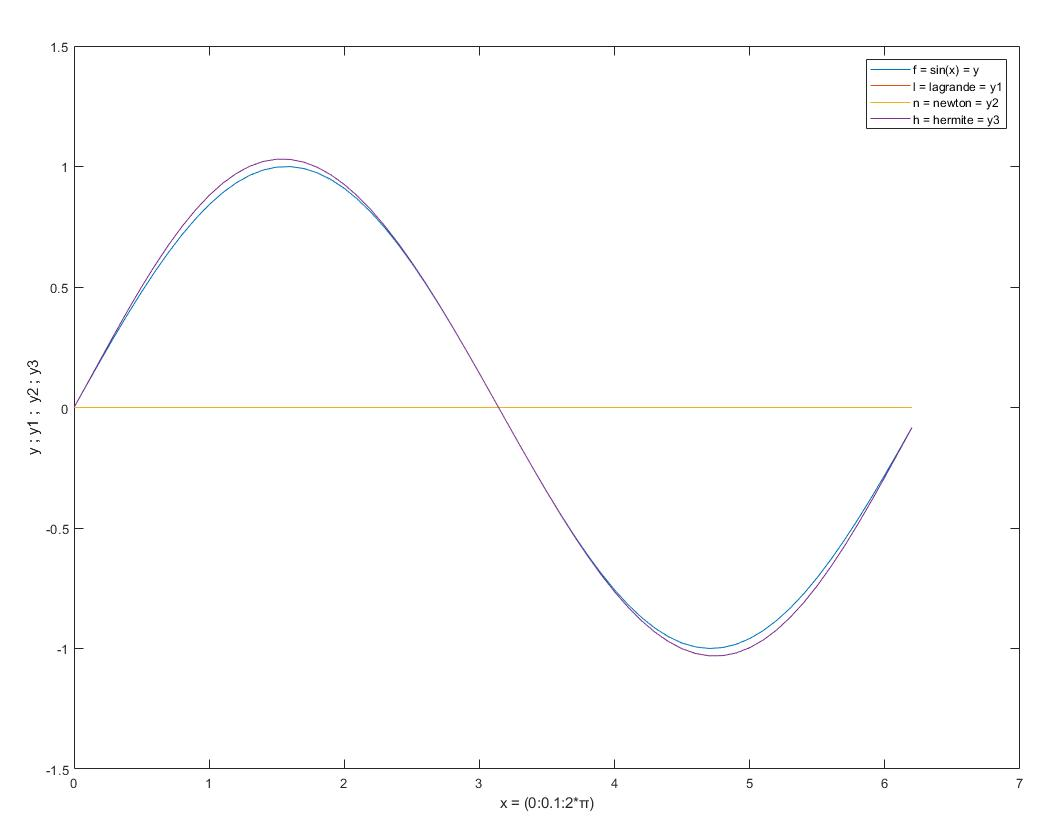
\includegraphics[width=\textwidth]{Plot/Cap_4_Es_4}
	\end{figure}
\newpage
\subsection{Esercizio 5}
Il seguente codice MatLab contiene l'implementazione della \textit{spline} cubica interpolante (naturale o \textit{not-a-knot}, come specificato in ingresso) delle coppie di dati assegnate. La forma della funzione è del tipo :\\ \textit{y = spline3( xi, fi, x, tipo )}.\\\
	\lstinputlisting[language=Matlab]{Cap_4/Es_5/spline3.m}
Da come si può vedere, all'interno del codice vengono richiamate le seguenti funzioni:\\\ 
	\begin{itemize}
		\item \textbf{dd = differenzaDivisa(xi, fi)}
	    	\lstinputlisting[language=Matlab]{Cap_4/Es_5/differenzaDivisa.m}
		\item \textbf{mi = risolviSistSplineNotAKnot(phi, xi, dd)}\\\
	    	\lstinputlisting[language=Matlab]{Cap_4/Es_5/risolviSistSplineNotAKnot.m}
		\item \textbf{mi = risolviSistSplineNaturale(phi, xi, dd)}\\\
	      	\lstinputlisting[language=Matlab]{Cap_4/Es_5/risolviSistSplineNaturale.m}
		\item \textbf{s = esprSpline3(xi, fi, mi)}\\\
	    	\lstinputlisting[language=Matlab]{Cap_4/Es_5/esprSpline3.m}
		\item \textbf{y = valutaSpline(xi, s, x)}\\\
	      	\lstinputlisting[language=Matlab]{Cap_4/Es_5/valutaSpline.m}
	\end{itemize}
Il seguente codice contiene il calcolo di una \textit{spline cubica}, basato sulla seguente funzione $y = \frac{1}{1+x^2}$.\\\
	\lstinputlisting[language=Matlab]{Cap_4/Es_5/Es_5.m}
	\begin{figure}[H]
		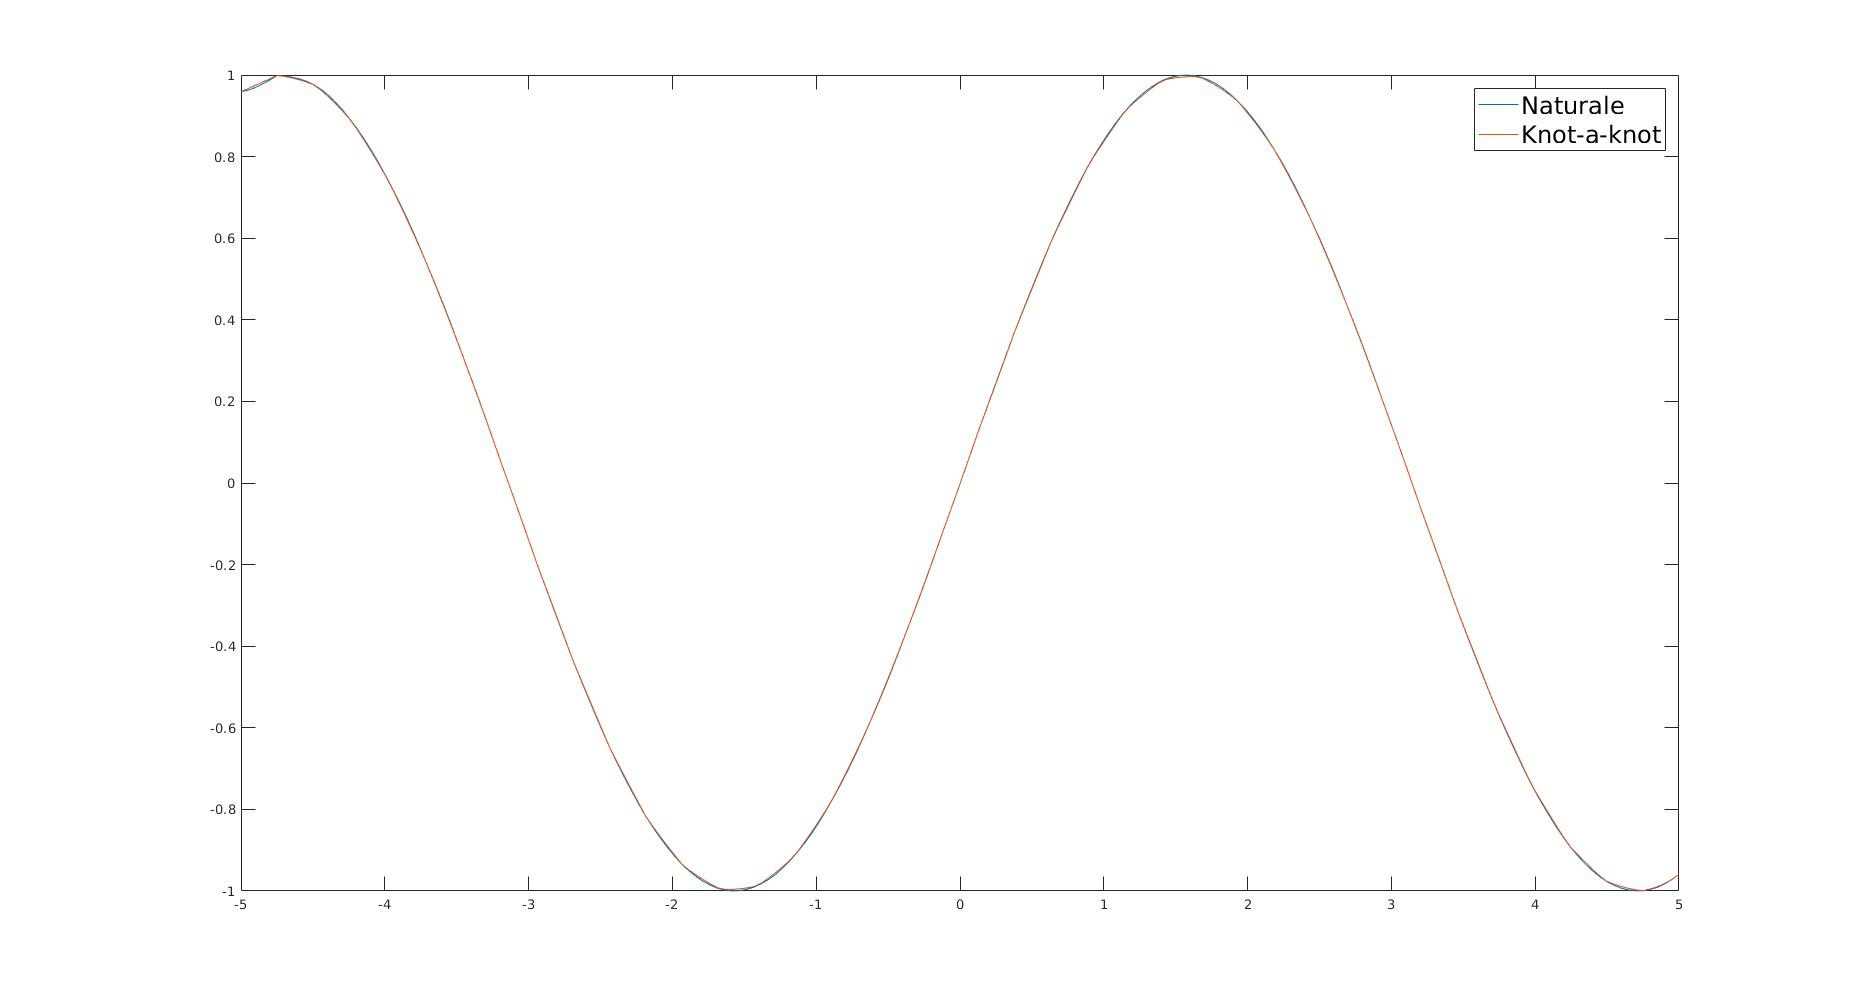
\includegraphics[width=\textwidth]{Plot/Cap_4_Es_5}
	\end{figure}

\newpage
\subsection{Esercizio 6}
Il seguente codice MatLab contiene l'implementazione del calcolo delle ascisse di Chebyshev per il polinomio interpolante di grado n, su un generico intervallo $[a,b]$. La forma della funzione è del seguente tipo: \textit{xi = ceby(n, a, b)}\\\
\lstinputlisting[language=Matlab]{Cap_4/Es_6/ceby.m}
\newpage
\subsection{Esercizio 7}
% Perchè non va, dio M..a?
\animategraphics[autoplay,loop,width=\textwidth]{100}{Gif/Cap_4_Es_7/runge-}{0}{108}

\newpage
\subsection{Esercizio 8}
Il seguente codice MatLab contiene la soluzione del problema dell'Es.8, che consiste nel calcolo della \textit{costante di Lebesgue}, la cui formula è la seguente:\\\
	\[
		\Lambda_n = ||\lambda_n|| \quad \lambda_n(x) = \sum_{k=0}^{n} |L_{(k,n)}(x)|
	\]
	\lstinputlisting[language=Matlab]{Cap_4/Es_8/Es_8.m}
In tale codice viene utilizzata la funzione \textit{leb = lebesgue(x)}:\\\
	\lstinputlisting[language=Matlab]{Cap_4/Es_8/lebesgue.m}
Nella seguente tabella è riportato come varia la \textit{costante di Lebesgue} $\Lambda$, al variare del grado \textit{n} del polinomio e si può notare come la crescita sia \textit{ottimale}, per $n\rightarrow\infty$:\\\
	\begin{center}
		\begin{tabular}{|c|c|}
			\hline
				$n$ & $\Lambda$ \\
    		\hline
    			$2$  & $1.250000000000000$ \\ 
    			$4$  & $1.570160602269766$ \\ 
    			$6$  & $1.782456998086407$ \\ 
    			$8$  & $1.941512423650456$ \\ 
    			$10$ & $2.068187442224371$ \\ 
    			$12$ & $2.174110871180027$ \\ 
    			$14$ & $2.264722328850426$ \\ 
    			$16$ & $2.343983362402486$ \\ 
   				$18$ & $2.409451754790443$ \\ 
    			$20$ & $2.469143366927380$ \\ 
    			$22$ & $2.528774997717951$ \\ 
    			$24$ & $2.588559223241643$ \\ 
    			$26$ & $2.623067061433159$ \\ 
    			$28$ & $2.670035980466209$ \\ 
    			$30$ & $2.726634058782908$ \\ 
    			$32$ & $2.747846892506189$ \\ 
    			$34$ & $2.785213548019579$ \\ 
    			$36$ & $2.820923625604030$ \\ 
    			$38$ & $2.855383873068024$ \\ 
    			$40$ & $2.886802263254646$ \\ 
			\hline
		\end{tabular}
	\end{center}

\newpage
\subsection{Esercizio 9}
%\lstinputlisting[language=Matlab]{Cap_4/Es_9/Es_9.m}

%\begin{figure}[H]
%	\label{Cap_4_Es_9}
%	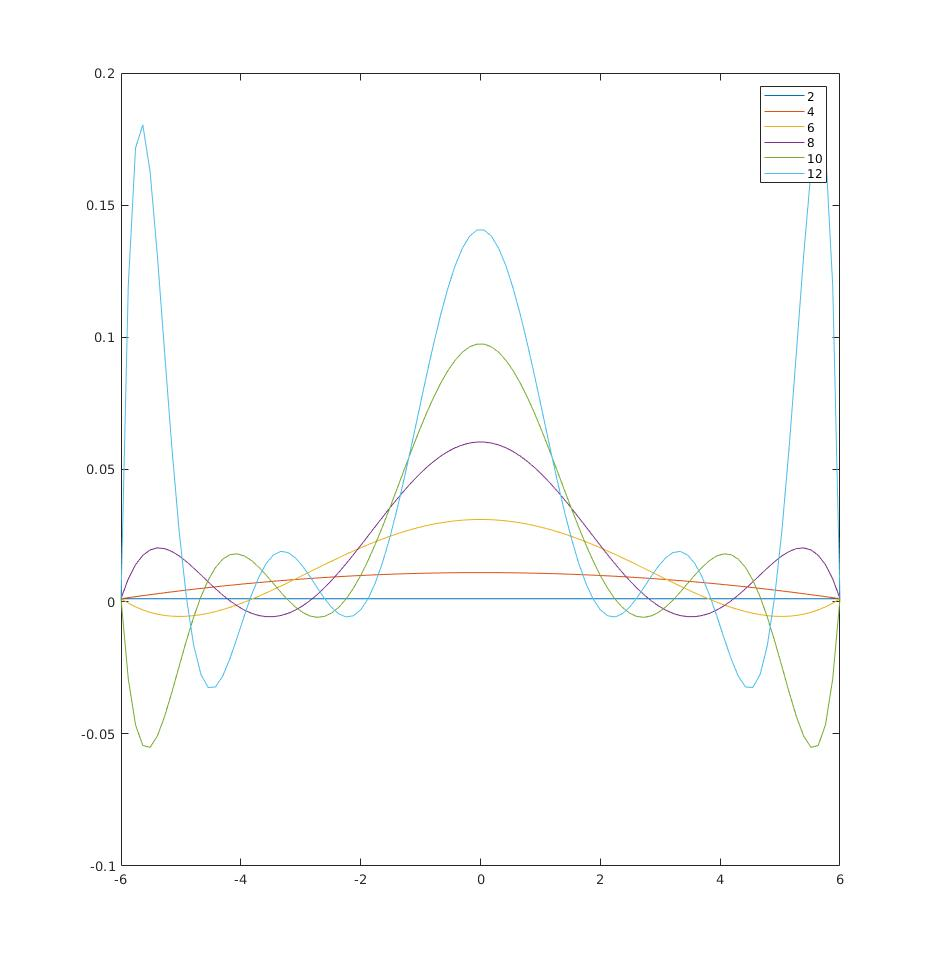
\includegraphics[width=\textwidth]{Plot/Cap_4_Es_9}
%	\caption{Polinomio di Lagrange con n° di ascisse $[2,4,6,8,10,12]$}
%\end{figure}

%\begin{figure}[H]
%	\label{Cap_4_Es_9(1)}
%	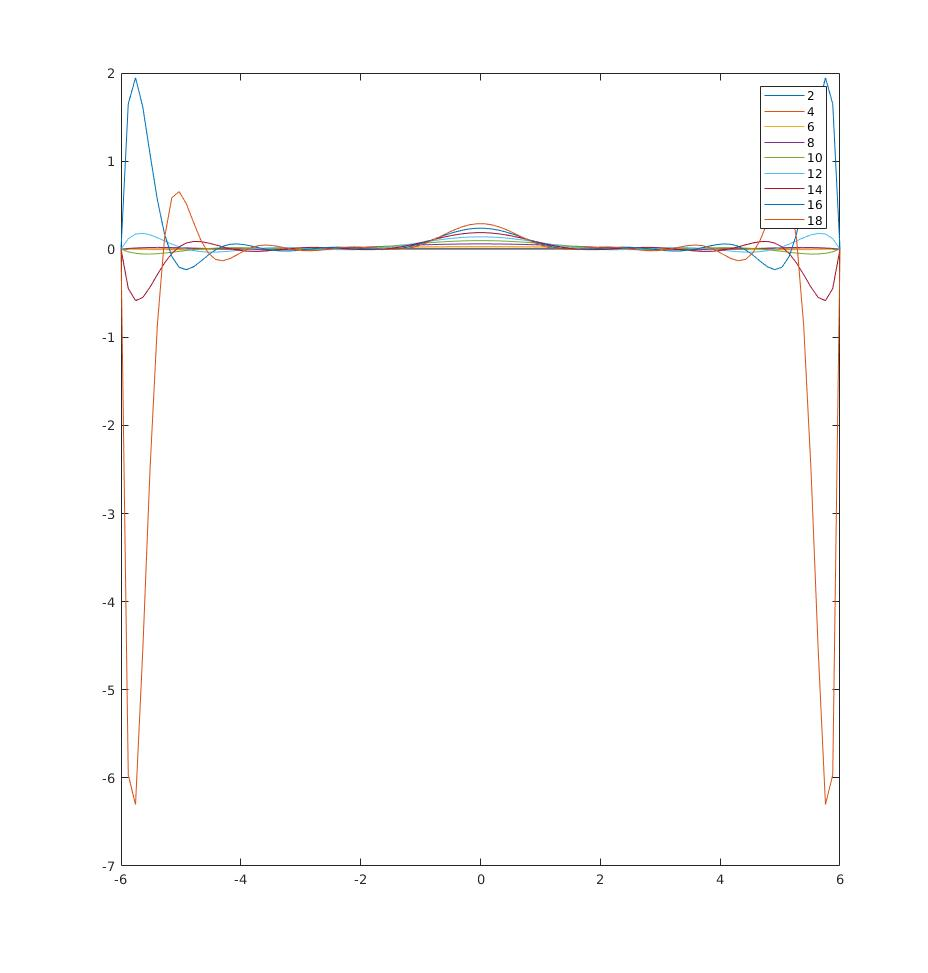
\includegraphics[width=\textwidth]{Plot/Cap_4_Es_9(1)}
%	\caption{Polinomio di Lagrange con n° di ascisse $[2,4,6,8,10,12,14,16,18]$}
%\end{figure}

%\begin{figure}[H]
%	\label{Cap_4_Es_9(2)}
%	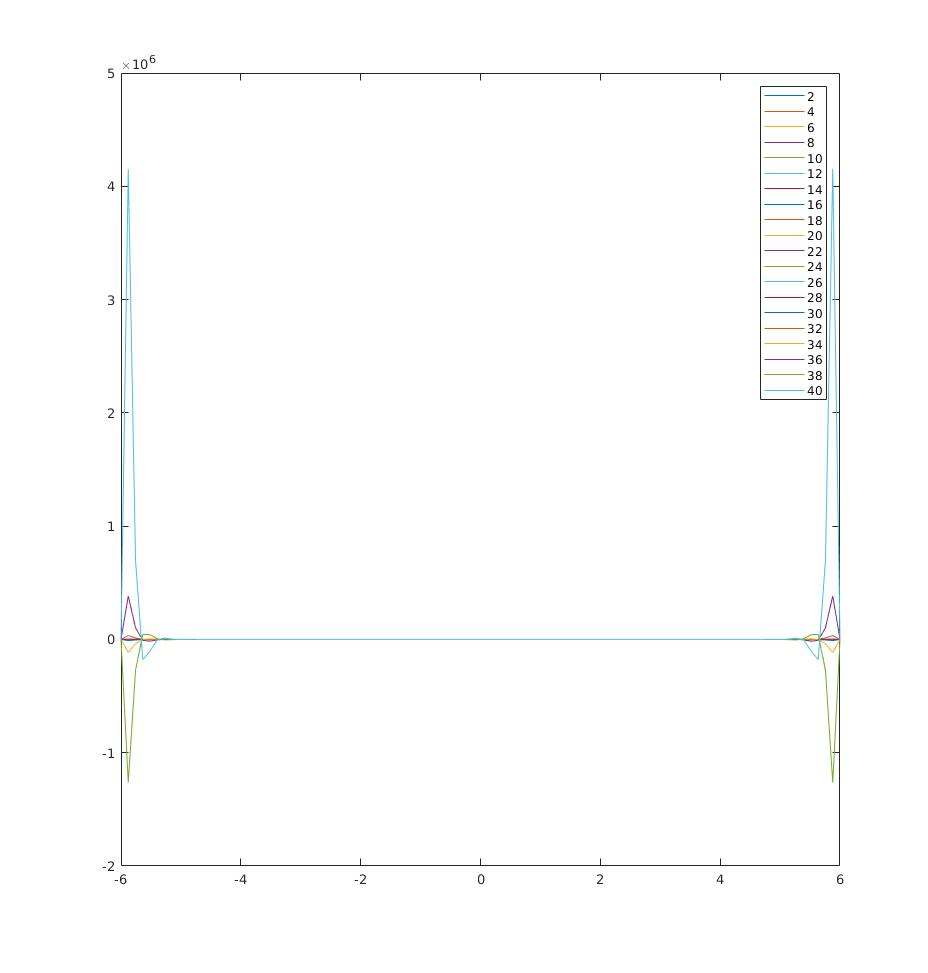
\includegraphics[width=\textwidth]{Plot/Cap_4_Es_9(2)}
%	\caption{Polinomio di Lagrange con n° di ascisse $[2,4,6,8,..,40]$}
%\end{figure}
\newpage
\subsection{Esercizio 10}
Il problema relativo ad un moto rettilineo uniformemente accelerato, in forma polinomiale è :
	\[
		x(t) = x_0 + v_0t + a_0t^2 \quad con \quad a_0 = \frac{1}{2}a
	\]
il cui grado è $n=2$.\\\
Il problema è \textit{ben posto}, cioè ammette soluzione ed è unica, se e solo se almeno $n+1$ ascisse $x_i$ delle coppie dei dati, sono tra loro distinte.\\\
Nel nostro caso, abbiamo le seguenti coppie di dati $(tempo, spazio)=(x_i,y_i)$ per $i=0,...,n$:\\\
	\[
		(1,2.9),(1,3.1),(2,6.9),(2,7.1),(3,12.9),(3,13.1),(4,20.9),(4,21.1),(5,30.9),(5,31.1)	
	\]\\\
quindi $x_i=5$ ascisse discinte che sono $\geq$ di $n+1 = 2+1 = 3$, di conseguenza il problema risulta \textit{ben posto}.\\\
A questo punto possiamo stimare, nel senso dei \textit{minimi quadrati},posizione, velocità iniziale, ed accelerazione, che equivale alla risoluzione del sistema lineare determinato:\\\
	\[
		V\underline{a}=\underline{y}
	\]
	\[
		V=\begin{bmatrix}
			x_0^0 & x_0^1 & \cdots & x_0^m \\
			x_1^0 & x_1^1 & \cdots & x_1^m \\
			\vdots & \vdots & & \vdots \\
			x_n^0 & x_n^1 & \cdots & x_n^m \\		
		\end{bmatrix}
		\quad
		\underline{a}=\begin{bmatrix}
			a_0 \\
			a_1 \\
			\vdots \\
			a_m
		\end{bmatrix}
		\quad
		\underline{y}=\begin{bmatrix}
			y_0 \\
			y_1 \\
			\vdots \\
			y_n
		\end{bmatrix}
	\]\\\
in cui la matrice dei coefficienti $V \in \mathbb{R}^{n+1Xm+1}$ è una matrice di tipo \textit{Vandermonde} (in realtà la trasposta di una matrice di tipo \textit{Vandermonde}), il vettore \underline{a}, è il vettore  da determinare e definisce il polinomio di approssimazione ai \textit{minimi quadrati}, ed infine il vettore \underline{y} è il vettore dei \textit{valori misurati}.\\\
Quindi scambiando le incognite con i valori di Input abbiamo che :\\\
	\[
		V=\begin{bmatrix}
			1^0 & 1^1 & 1^2 \\
			1^0 & 1^1 & 1^2 \\
			2^0 & 2^1 & 2^2 \\
			2^0 & 2^1 & 2^2 \\
			3^0 & 3^1 & 3^2 \\
			3^0 & 3^1 & 3^2 \\
			4^0 & 4^1 & 4^2 \\
			4^0 & 4^1 & 4^2 \\
			5^0 & 5^1 & 5^2 \\
			5^0 & 5^1 & 5^2 				
		\end{bmatrix}
		=\begin{bmatrix}
			1 & 1 & 1 \\
			1 & 1 & 1 \\
			1 & 2 & 4 \\
			1 & 2 & 4 \\
			1 & 3 & 9 \\
			1 & 3 & 9 \\
			1 & 4 & 16 \\
			1 & 4 & 16 \\
			1 & 5 & 25 \\
			1 & 5 & 25 				
		\end{bmatrix} 
		\quad
		\underline{a}=\begin{bmatrix}
			x_0 \\
			v_0 \\
			a_0
		\end{bmatrix}
		\quad
		\underline{y}=\begin{bmatrix}
			2.9 \\
			3.1 \\
			6.9 \\
			7.1 \\
			12.9 \\
			13.1 \\
			20.9 \\
			21.1 \\
			30.9 \\
			31.1
		\end{bmatrix}
	\]\\\
ed il sistema lineare sovradeterminato da risolvere è :\\\
	\[
		\begin{bmatrix}
			1 & 1 & 1 \\
			1 & 1 & 1 \\
			1 & 2 & 4 \\
			1 & 2 & 4 \\
			1 & 3 & 9 \\
			1 & 3 & 9 \\
			1 & 4 & 16 \\
			1 & 4 & 16 \\
			1 & 5 & 25 \\
			1 & 5 & 25 				
		\end{bmatrix}
		\begin{bmatrix}
			x_0 \\
			v_0 \\
			a_0
		\end{bmatrix}=
		\begin{bmatrix}
			2.9 \\
			3.1 \\
			6.9 \\
			7.1 \\
			12.9 \\
			13.1 \\
			20.9 \\
			21.1 \\
			30.9 \\
			31.1
		\end{bmatrix}
	\]\\\
Tale sistema si risolve mediante fattorizzazione \textit{QR} (possibile poichè tutte le ascisse sono distinti).
Il seguente codice MatLab contiene la chiamata della funzione \textit{risolutoreQR} con Input la matrice $V$ e il vettore dei termini noti $b$:
	\lstinputlisting[language=Matlab]{Cap_4/Es_10/Es_10.m}
restituendo i seguenti risultati (vettore da determinare $\underline{a}$ e il vettore \textit{residuo} $\underline{r}$ e la rispettiva \textit{norma}):
	\[
		\underline{a}=\begin{bmatrix}
			1.000000000000001e+00 \\
			1.000000000000002e+00 \\
	 	    9.999999999999994e-01
		\end{bmatrix}
		\quad
		\underline{r}=\begin{bmatrix}
			1.000000000000023e-01 \\
   			-9.999999999999787e-02 \\
     		1.000000000000032e-01 \\
    		-9.999999999999609e-02 \\
     		1.000000000000014e-01 \\
    		-9.999999999999787e-02 \\
     		1.000000000000014e-01 \\
    		-1.000000000000014e-01 \\
     		9.999999999999787e-02 \\
    		-1.000000000000050e-01
		\end{bmatrix}
		\quad
		\|r\|_2^2 = 1.000000000000009e-01
	\]
\newpage
\newpage
\section{\textbf{Capitolo 5}}

\newpage
\section{\textbf{Capitolo 6}}
\subsection{Esercizio 1}
Il seguente codice MatLab contiene l'implementazione della funzione \textit{S=sparseMatrix(n)} :\\\
	\lstinputlisting[language=Matlab]{Cap_6/Es_1/sparseMatrix.m}
il quale restituisce una \textit{matrice sparsa} $nXn$ della forma:\\\
	\[
		S=A_n=\begin{pmatrix}
			a_{11} & \cdots & a_{1n} \\
			\vdots &		& \vdots \\
			a_{n1} & \cdots & a_{nn} 
		\end{pmatrix}
	\quad
		a_{ij}=\begin{cases}
				 4 \textit{ se } i=j \\ -1 \textit{  se } i=j\pm1 \\  -1 \textit{  se } i=j\pm10
				\end{cases}
	\]
\newpage
\subsection{Esercizio 2}
Il seguente codice MatLab contiene la soluzione dell'$Es 2$:\\\
	\lstinputlisting[language=Matlab]{Cap_6/Es_2/Es_2.m}
nel qualche viene richiamato:\\\
	\begin{enumerate}
		\item \textbf{A = sparceMatrix(n)}\\\
			Effettua la creazione di \textit{matrici sparse} della dimensione $nXn$;\\\
		\item \textbf{y,i = potenze(A,tol)}\\\
			Effettua sia il calcolo dell'\textit{autovalore} della matrice $A$, sia il numero di iterazioni impiegate, avendo come \textit{Input}, oltre la 	\textit{matrice} e la \textit{tolleranza}, anche un \textit{vettore iniziale ad elementi costanti}.\\\
			\lstinputlisting[language=Matlab]{Cap_6/Es_2/potenze.m}	
	\end{enumerate}
e restituisce i seguenti risultati:\\\
	\begin{center}
		\begin{tabular}{|c|c|c|}
			\hline
				$n$ & \textit{numero iterazioni effettuate} & \textit{stima autovalore} \\
			\hline
				$100$ & $167$ & $7.822407378611797$ \\
				$200$ & $420$ & $7.880289827977503$ \\
				$300$ & $638$ & $7.891572462961987$ \\
				$400$ & $721$ & $7.894873000091178$ \\
				$500$ & $743$ & $7.896381732961388$ \\
				$600$ & $824$ & $7.897427743600915$ \\
				$700$ & $893$ & $7.897595598256215$ \\
				$800$ & $868$ & $7.896679356756460$ \\
				$900$ & $795$ & $7.895666037100858$ \\
				$1000$ & $775$ & $7.895414407762564$ \\
			\hline 
		\end{tabular}
	\end{center}
\newpage
\subsection{Esercizio 3}
Il seguente codice MatLab contiene la soluzione dell'$Es 3$:\\\
	\lstinputlisting[language=Matlab]{Cap_6/Es_3/Es_3.m}
nel qualche viene richiamato:\\\
	\begin{enumerate}
		\item \textbf{A = sparceMatrix(n)}\\\
			Effettua la creazione di \textit{matrici sparse} della dimensione $nXn$;\\\
		\item \textbf{y,i = jacobi(A,b,tol,x0)}\\\
			Effettua sia il calcolo del \textit{vettore incognite} della matrice $A$, sia il numero di iterazioni impiegate, avendo come \textit{Input}, oltre la 	\textit{matrice}, il \textit{vettore termini noti}, e la \textit{tolleranza}, anche un \textit{vettore iniziale, in questo cado nullo}.\\\
			\lstinputlisting[language=Matlab]{Cap_6/Es_3/jacobi.m}
	\end{enumerate}
e restituisce graficamente i seguenti risultati:\\\
	\begin{figure}[H]
		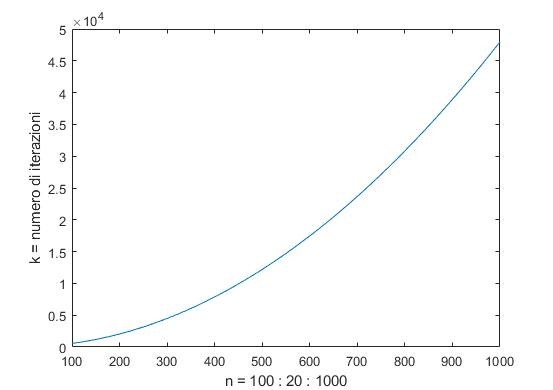
\includegraphics[width=\textwidth]{Plot/Cap_6_Es_3}
	\end{figure}
\newpage
\subsection{Esercizio 4}
Il seguente codice MatLab contiene la soluzione dell'$Es 4$:\\\
\lstinputlisting[language=Matlab]{Cap_6/Es_4/Es_4.m}
nel qualche viene richiamato:\\\
\begin{enumerate}
	\item \textbf{A = sparceMatrix(n)}\\\
		Effettua la creazione di \textit{matrici sparse} della dimensione $nXn$;\\\
	\item \textbf{y,i = gaussSeidel(A,b,tol,x0)}\\\
		Effettua sia il calcolo del \textit{vettore incognite} della matrice $A$, sia il numero di iterazioni impiegate, avendo come \textit{Input}, oltre la 	\textit{matrice}, il \textit{vettore termini noti}, e la \textit{tolleranza}, anche un \textit{vettore iniziale, in questo cado nullo}.\\\
		\lstinputlisting[language=Matlab]{Cap_6/Es_4/gaussSeidel.m}
	\begin{itemize}
		\item \textbf{u = mSolve(M,r)}\\\
			Effettua il calcolo di una matrice \textit{triangolare inferiore}.\\\
			\lstinputlisting[language=Matlab]{Cap_6/Es_4/mSolve.m}
	\end{itemize}
\end{enumerate}
e restituisce graficamente i seguenti risultati:\\\

\newpage
\subsection{Esercizio 5}
Il seguente codice MatLab contiene la soluzione dell'$Es 5$:\\\
	\lstinputlisting[language=Matlab]{Cap_6/Es_5/Es_5.m}
nel qualche viene richiamato:\\\
	\begin{enumerate}
		\item \textbf{A = sparceMatrix(n)}\\\
			Effettua la creazione di \textit{matrici sparse} della dimensione $nXn$;\\\
		\item \textbf{y,B = jacobi(A,b,tol,x0)}\\\
			Effettua sia il calcolo del \textit{vettore incognite} della matrice $A$, sia il calcolo di una matrice $B$ contenente il \textit{passo di ogni iterazione} con il corrispettivo \textit{valore della norma}, avendo come \textit{Input}, oltre la \textit{matrice}, il \textit{vettore termini noti}, e la \textit{tolleranza}, anche un \textit{vettore iniziale, in questo caso nullo}.\\\
		\item \textbf{y,B = gaussSeidel(A,b,tol,x0)}\\\
			Effettua sia il calcolo del \textit{vettore incognite} della matrice $A$, sia il calcolo di una matrice $B$ contenente il \textit{passo di ogni iterazione} con il corrispettivo \textit{valore della norma}, avendo come \textit{Input}, oltre la 	\textit{matrice}, il \textit{vettore termini noti}, e la \textit{tolleranza}, anche un \textit{vettore iniziale, in questo cado nullo}.\\\
		\begin{itemize}
			\item \textbf{u = mSolve(M,r)}\\\
				Effettua il calcolo di una matrice \textit{triangolare inferiore}.\\\
		\end{itemize}
	\end{enumerate}
e restituisce graficamente i seguenti risultati:\\\
	\begin{figure}[H]
		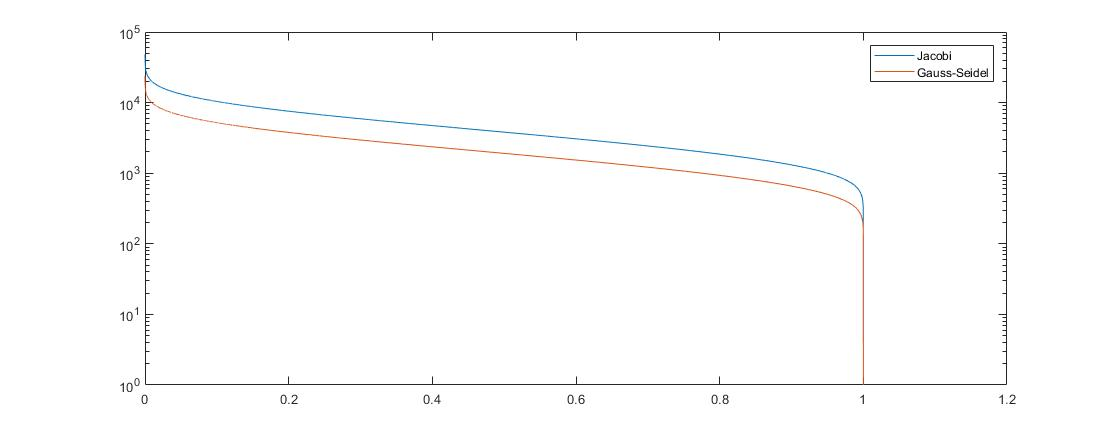
\includegraphics[width=\textwidth]{Plot/Cap_6_Es_5}
	\end{figure}
\newpage
\newpage
\end{document}